\documentclass[10.5pt]{article}

\usepackage[left=2cm, right=2cm, top=3cm, bottom = 3cm]{geometry}

\usepackage{color}
\usepackage{amsmath}
\usepackage{amsfonts}
\usepackage{amssymb}
\usepackage{graphicx}
\usepackage{float}
\usepackage{indentfirst}
\usepackage{wrapfig}
\usepackage{latexsym}
\usepackage{hyperref}
\usepackage[export]{adjustbox}
\usepackage{physics}
\usepackage{bbold}
\usepackage{extarrows}
\usepackage{listings}
\usepackage{multirow}
\usepackage [english]{babel}
\usepackage{natbib}
\bibliographystyle{plain}


\linespread{1.2}
\newcommand{\Hami}{\mathcal{H}}
\newcommand{\R}{\mathcal{R}}


\author{Xu-Yao Hu\\ Department of Physics, New York University}
\title{\bf{Computational Physics Final Project \\1D MHD code building and testing}}
\date{\today}

\begin{document}
\maketitle
\begin{abstract}
	A one-dimensional MHD code using PLM + HLLD is constructed. 
	Compared to the code with the
	regular HLL scheme, the code based on HLLD is confirmed to be less diffusive, which 
	indicates that HLLD scheme is more advanced and more suitable to be applied in 
	MHD code.
	Several shock tube tests, rarefaction wave tests are performed to examine the effectiveness 
	and the accuracy of my MHD code. The results given by 
	my MHD code agree with those presented in previous papers. A sinusoidal Alfv\'en wave 
	example is constructed using my MHD code. 
	The wave speed of the constructed Alfv\'en wave 
	obtained using my MHD code is consistent with the theoretical expectation.
	An animation of Alfv\'en Wave is generated, which presents a
	more clear scenario of this dynamical process.
\end{abstract}

\section{Introduction}
Magnetohydrodynamics (MHD) is extremely important in various fields such as Astrophysics, Geophysics and Plasma Physics.

The thrust of this work is to construct a reliable 1D MHD code by using higher-order Piecewise 
Linear Method (PLM) and Harten-Lax-van Leer (HLL) type Riemann Solvers. 
We attempt to construct both PLM + regular HLL code and PLM + HLLD code, and 
run several test problems to check the effectiveness and the accuracy of the code.

For an ideal MHD system,
the basic dynamics equations are the mass conservation equation, 
the momentum conservation equation, the energy conservation equation, 
and Ohm's law with Maxwell's Equations. All equations can be written in conservative form as
 (See \cite{stone2008athena})
 \begin{align}
 	&\pdv{\rho}{t}+\div (\rho \vb*{v})=0 \ , \\
	&\pdv{\rho \vb*{v}}{t} +\div (\rho \vb*{v}\vb*{v}-\vb*{B}\vb*{B}+\vb*{P}_T)=0 \ , \\
	&\pdv{E}{t} + \div [(E+P_T)\vb*{v}-\vb*{B}(\vb*{B}\vdot\vb*{v})]=0 \ , \\
	&\pdv{\vb*{B}}{t}-\curl (\vb*{v} \cross \vb*{B})=0 \ .
 \end{align}
 where $\rho$ is the fluid mass density, $\vb*{v}=(v_x,v_y,v_z)$ is the flow velocity, $\vb*{B}$ is the magnetic field, 
 $E$ is the total energy density,
 $\vb*{P}_T \equiv P_T \vb*{I}$ is a diagonal tensor with components 
 $P_T=P+\frac{1}{2}B^2$ with $P$ being the pressure. The equations above are written in 
 units such that the magnetic permeability $\mu=1$.
To close the equations, we usually need the equation of state (EoS) for ideal fluid (gas). 
Actually, EoS can be encoded in the expression of the total energy density 
\begin{align}
	E=\frac{P}{\gamma-1}+\frac{1}{2}\rho v^2+\frac{B^2}{2} \ ,
\end{align}
where $\gamma$ is the adiabatic index of the ideal gas.
It is useful to write down the explicit form of the thermodynamical pressure
\begin{align}
	P=(\gamma-1)\left[E-\frac{1}{2}\rho v^2-\frac{B^2}{2}\right] \ .
\end{align}

\section{Numerical Method}
\subsection{1D MHD in Cartesian coordinates}
The project starts with solving 1D effective problems (all physical quantities depend on 
one position component, say $x$, and time $t$). 
The 1D MHD equations can be cast into a compact form as 
\begin{align}
	\pdv{\vb*{U}}{t}+\pdv{\vb*{F}}{x}=0 \ ,
\end{align}
where $\vb*{U}$ and $\vb*{F}$ are the vectors 
of all conserved 
variables and fluxes in Cartesian coordinates respectively and given by
$\vb*{U}=(\rho,\rho v_x, \rho v_y, \rho v_z, E, B_x, B_y, B_z)^T$ and 
$\vb*{F}=(\rho v_x, \rho v_x^2 + P_T -B_x^2,\rho v_x v_y - B_x B_y, \rho v_x v_z - B_x B_z, (E+P_T)v_x - (\vb*{B}\vdot\vb*{v}) B_x, 0, B_y v_x - B_x v_y, B_z v_x - B_x v_z)^T$. 
Since the sixth pair of components are trivial in 1D case ($B_x=\text{constant}$), 
we use the simplified form of the 
vectors for 1D code as follows,
\begin{align}
	\vb*{U}=\begin{pmatrix}
	\rho \\
	\rho v_x \\
	\rho v_y \\
	\rho v_z \\
	E \\
	B_y \\
	B_z
	\end{pmatrix} \ , 
	\qquad 
	\vb*{F}=\begin{pmatrix}
	\rho v_x \\
	\rho v_x^2 + P_T -B_x^2 \\
	\rho v_x v_y - B_x B_y \\
	\rho v_x v_z - B_x B_z \\
	(E+P_T)v_x - (\vb*{B}\vdot\vb*{v}) B_x \\
	B_y v_x - B_x v_y \\
	B_z v_x - B_x v_z
	\end{pmatrix} \ .
\end{align}
It is often useful to introduce the vector of primitive variables:
\begin{align}
	\vb*{Q}=\begin{pmatrix}
		\rho \\
		v_x \\
		v_y \\
		v_z \\
		P \\
		B_y \\
		B_z
	\end{pmatrix} \ .
\end{align}


\subsection{Algorithm}
The algorithm of my 1D MHD code is described in details in this section.
\begin{enumerate}
	\item [\textbf{Step 1}] Input the initial conditions of the MHD system and write them in 
	terms of the conserved variable vector $\vb*{U}$ and the fluxes vector $\vb*{F}$.

	\item [\textbf{Step 2}] Construct the ``left'' and ``right'' states at every interface using 
	Piecewise Linear Method (PLM) [This part is done by \texttt{PLM} function in 
	\texttt{MHD\_1d\_Solver\_Scheme.py}.]
	\begin{enumerate}
		\item Receive $\vb*{U}$ vector (for each cell center) and 
		convert it into $\vb*{Q}$ vector (for each cell center);\\
		\textbf{Technicall details:}  Both $\vb*{U}$ and $\vb*{Q}$ are $7\times (N+4)$ 
		matrices with
	 	$i=2,3,\cdots N+1$ representing real cells ($N$ real cells in total) 
	 	and $i=0,1,N+2,N+3$ denoting ghost cells.
		\item Using PLM to get $\vb*{Q}_L$ (for each interface) and $\vb*{Q}_R$ 
		(for each interface) from $\vb{Q}$ (for each cell center);\\
	 	\textbf{Technical details:} To make things easy to track, we also set $\vb*{Q}_L$ and 
	 	$\vb*{Q}_R$ as $7\times (N+4)$ matrices with $i=1,2,\cdots,N+1$ are real interfaces 
	 	that we're interested in and $i=0,N+2,N+3$ being spare interfaces on 
		which no operation is performed. 
		By ``real'' interfaces, I refer to the interfaces which are the boundaries 
	of the real cells.
		\item Calculate the fast magneto-acoustic wave speeds for the ``left'' and ``right'' states,
		 i.e. $c_{fL}$ and $c_{fR}$ using the following equation:
			\begin{align}
				c_f = \left[\frac{\gamma P + |\vb*{B}|^2 + \sqrt{(\gamma P + |\vb*{B}|^2)^2 - 
				4\gamma P B_x^2}}{2\rho}\right]^{1/2} \ ,
			\end{align}
		thus obtaining the smallest and the largest eigenvalues $\lambda_1 = v_x - c_f$ and 
		$\lambda_7 = v_x + c_f$ for the ``left'' and ``right'' states.
		\item Determine the minimum and maximum signal speed as 
			\begin{align}
				&S_L = \min[\lambda_1(\vb*{U}_L),\lambda_1({\vb*{U}_R})] \ , \\
				&S_R = \max[\lambda_7(\vb*{U}_L),\lambda_7({\vb*{U}_R})] \ .
			\end{align}
	\end{enumerate}
	
	\item[\textbf{Step 3}] Compute the flux at each real interface using a HLL-type 
	Riemann Solver\footnote{For more details about HLL and HLLD, 
	see Mitoshi \& Kusano \cite{miyoshi2005multi}} (This part is done by functions
	\texttt{F\_HLL\_generator} and \texttt{F\_HLLD\_generator} in
	\texttt{MHD\_1d\_Solver\_Scheme.py})
	\begin{itemize}
		\item For HLL Solver:\\
			Calculate the intermediate fluxes $\vb*{F}^*$ and the HLL fluxes is given by 
			\begin{align}
			\vb*{F}_{\text{HLL}} = \begin{cases}
				\vb*{F}_{\text{L}} & \text{if } S_L>0 \ ,  \\
				\vb*{F}^* & \text{if } S_L \leq 0 \leq S_R \ , \\
				\vb*{F}_{\text{R}} & \text{if } S_R<0 \ .
				\end{cases}
			\end{align}	
		\item For HLLD Solver:\\
			Calculate the intermediate fluxes $\vb*{F}_L^*$, 
			$\vb*{F}_L^{**}$, $\vb*{F}_R^*$, $\vb*{F}_R^{**}$  and the HLLD fluxes is given by 
			\begin{align}
				\vb*{F}_{\text{HLLD}} = \begin{cases}
				\vb*{F}_{\text{L}} & \text{if } S_L>0 \ ,  \\
				\vb*{F}^*_{\text{L}} & \text{if } S_L \leq 0 \leq S^*_L \ , \\
				\vb*{F}^{**}_{\text{L}} & \text{if } S^*_L \leq 0 \leq S_M \ , \\
				\vb*{F}^{**}_{\text{R}} & \text{if } S_M \leq 0 \leq S^*_R \ , \\
				\vb*{F}^{*}_{\text{R}} & \text{if } S^*_R \leq 0 \leq S_R \ , \\
				\vb*{F}_{\text{R}} & \text{if } S_R<0 \ .
				\end{cases}
			\end{align}	
	\end{itemize}
	\item[\textbf{Step 4}] Update the cell-centered conserved variables using the third-order 
	Runge-Kutta scheme devised by Shu \& Osher:
	\begin{align}
	\vb{U}^{(1)}&=\vb{U} + \Delta t L(\vb{U}^n) \ , \\
	\vb{U}^{(2)} &= \frac{3}{4} \vb{U}^n + \frac{1}{4} \vb{U}^{(1)}+\frac{1}{4}\Delta t L(\vb{U}^{(1)}) 	\ , \\
	\vb{U}^{n+1}&=\frac{1}{3} \vb{U}^n + \frac{2}{3} \vb{U}^{(2)} +\frac{2}{3}\Delta t L(\vb{U}^{(2)}) 	\ ,
	\end{align}
	where $L(\vb*{U_i}) = -\frac{\vb*{F}_{\text{HLLD},i+1/2} - \vb*{F}_{\text{HLLD},i-1/2}}
	{\Delta x}$ for HLLD fluxes and $\Delta t$ is determined by CFL stability condition
	\begin{align}
		\Delta t = C_{\text{CFL}} \Delta x/\max (v^n_{x,i} + c^n_{f,i})\ ,
	\end{align}
	where $C_{\text{CFL}}<1$ is referred to as CFL number.
\end{enumerate}


\section{Numerical Tests}
All relevant numerical test results and discussions of my 1d MHD code are elaborated in 
this section.
\subsection{Dai \& Woodward shock tube test}
Dai \& Woodward (1994) \cite{DW1994} proposed a typical one-dimensional 
shock tube problem, which was solved by Miyoshi \& Kusano \cite{miyoshi2005multi}
in the interval $x\in[-0.5,0.5]$ with 800 cells and CFL number 
$0.8$. The initial conditions ($t=0$) are given by 
\begin{align}
&(\rho,\ P,\ v_x,\ v_y,\ v_z,\ B_y,\ B_z) = (1.08, 0.95, 1.2, 0.01, 0.5, 3.6/\sqrt{4 \pi}, 2/\sqrt{4\pi}) \quad
\text{for } x<0 \ , \\
&(\rho,\ P,\ v_x,\ v_y,\ v_z,\ B_y,\ B_z) = (1, 1, 0, 0, 0, 4/\sqrt{4 \pi}, 2/\sqrt{4\pi}) \quad
\text{for } x>0  \ , 
\end{align}
with $B_x = 4/\sqrt{4\pi}$.
The exact solution of this shock tube problem includes several shocks and discontinuities: 
two fast shocks, two rotational discontinuities, two slow shocks, and a contact discontinuity.

Fig. \ref{fig: DW shock test} shows the distribution of all physical quantities at time $t=0.2$. 
The zoomed-in graphs confirms the statement that the regular HLL scheme is more diffusive than 
the HLLD scheme. My code indeed captures all the features of Dai \& Woodward shock 
as did by Miyoshi \& Kusano \cite{miyoshi2005multi}.

\begin{figure}[ht]
	\centering
	\begin{minipage}[c]{0.9\textwidth}
		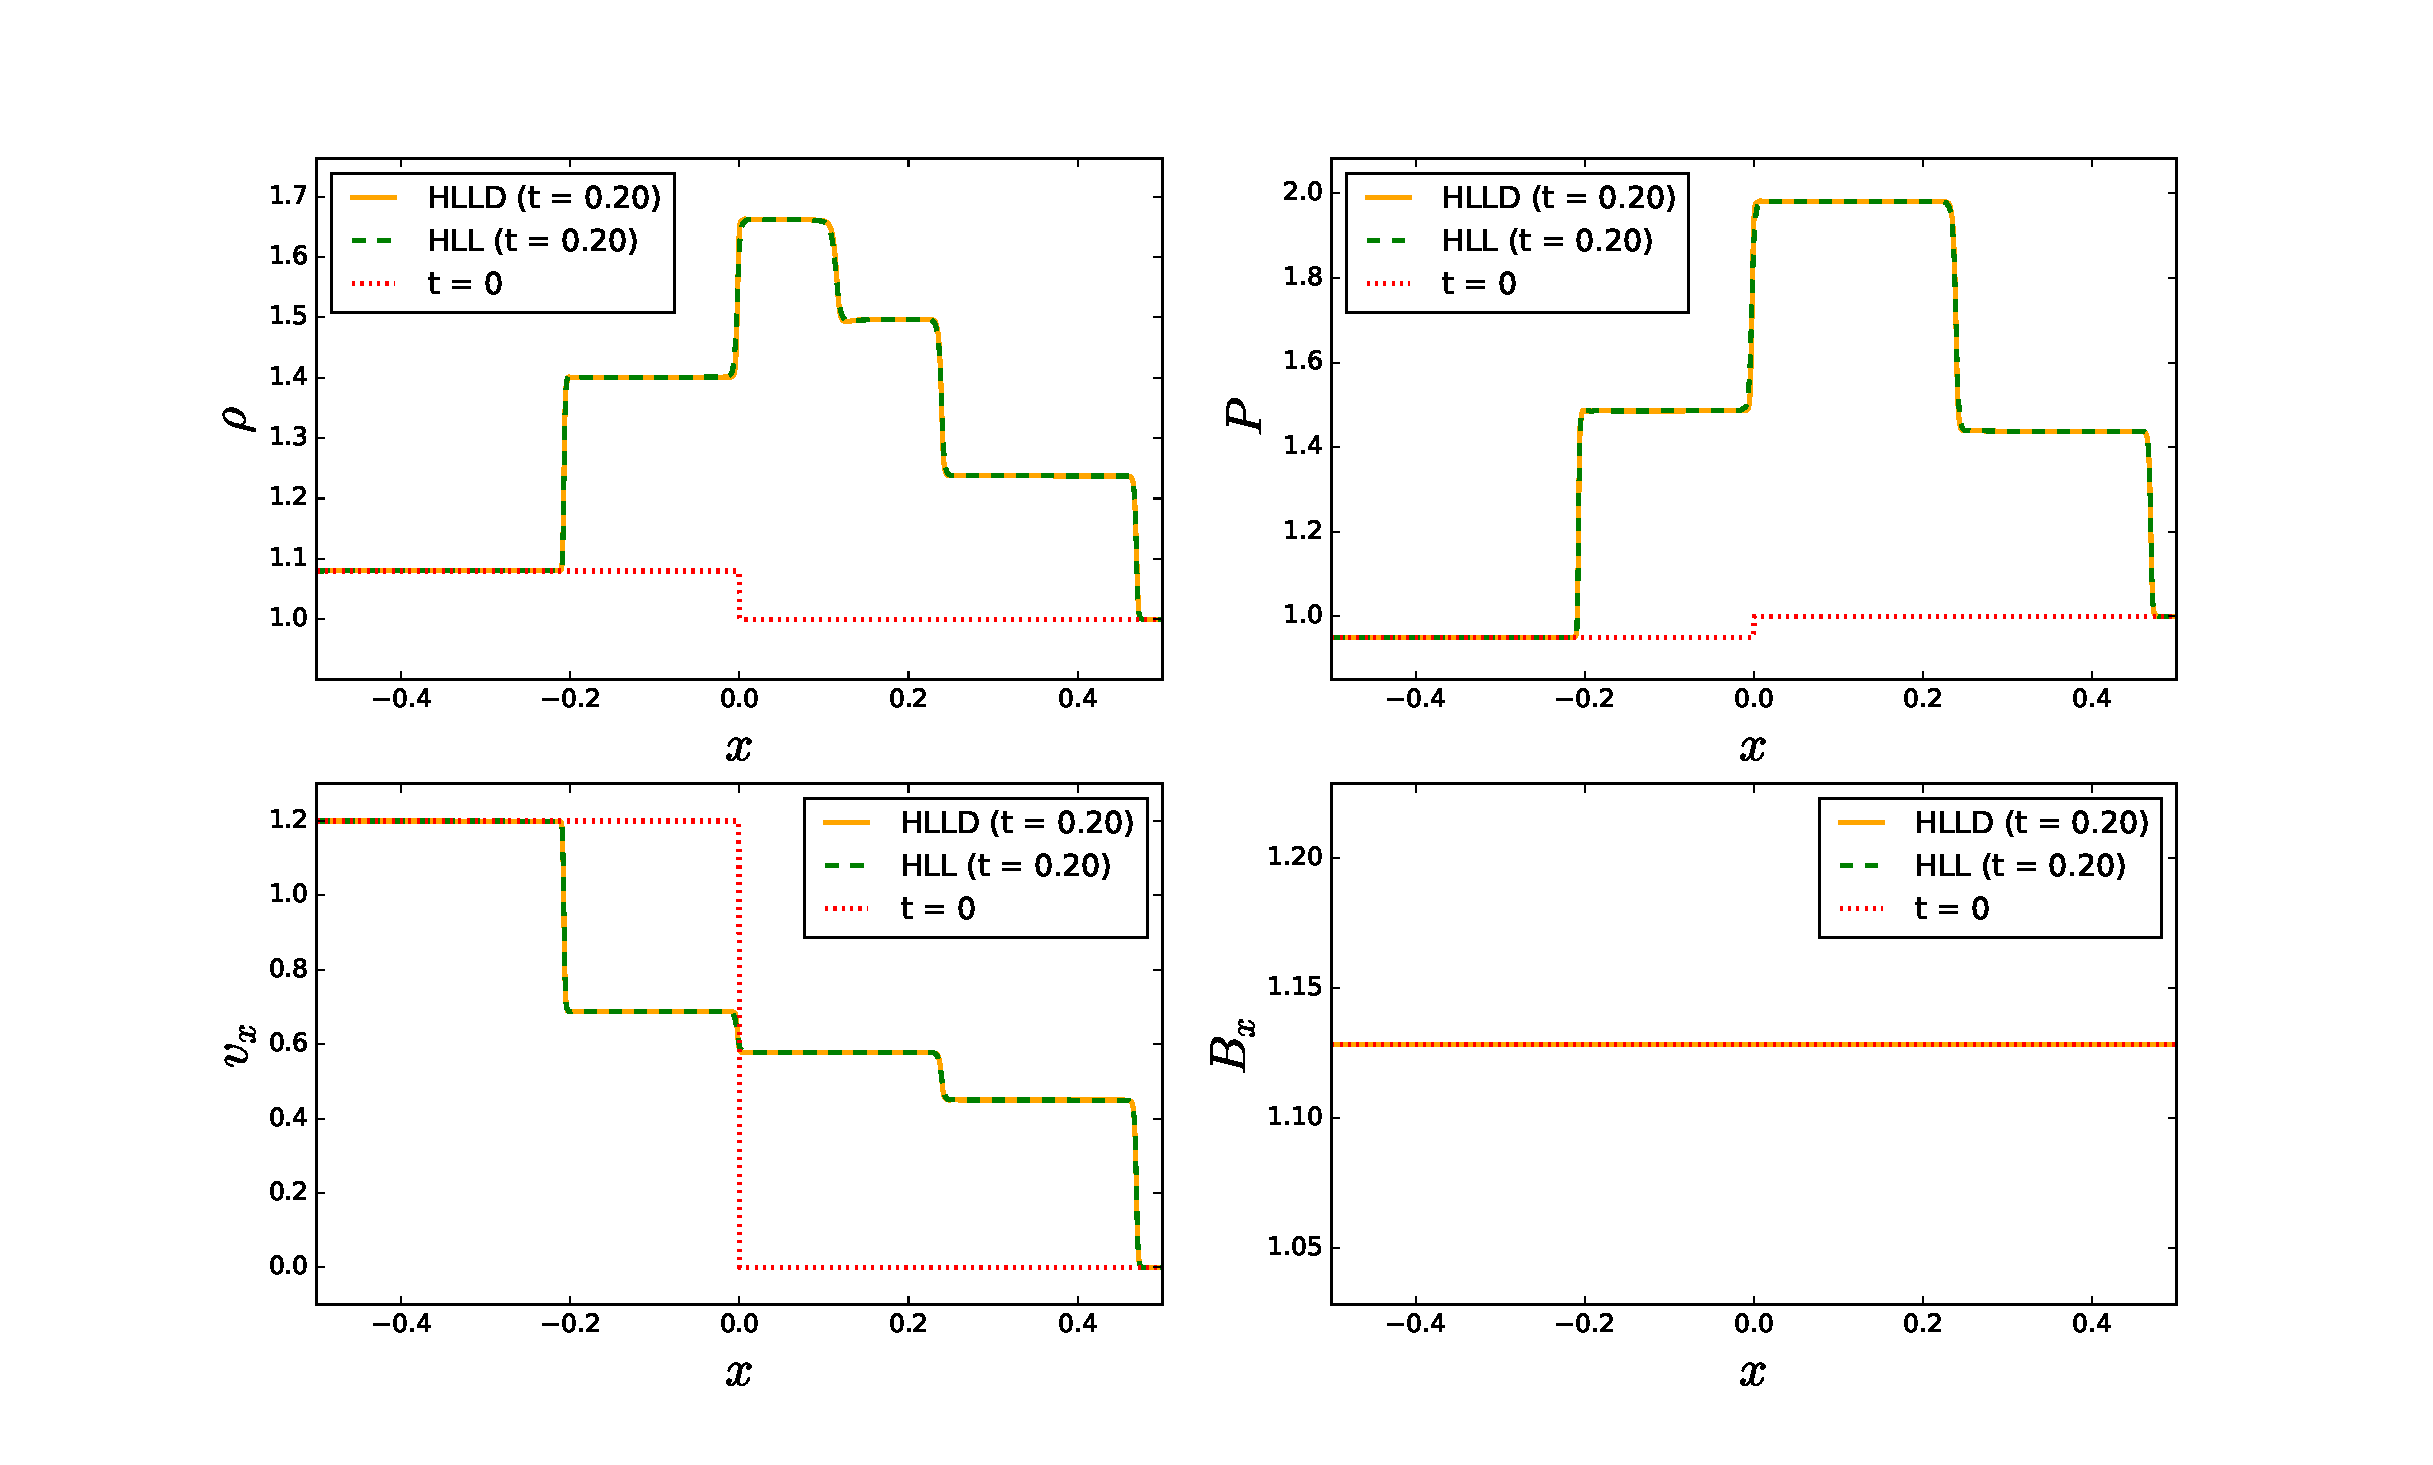
\includegraphics[width=1\textwidth]{DW1.eps}
	\end{minipage}
	\begin{minipage}[c]{0.9\textwidth}
		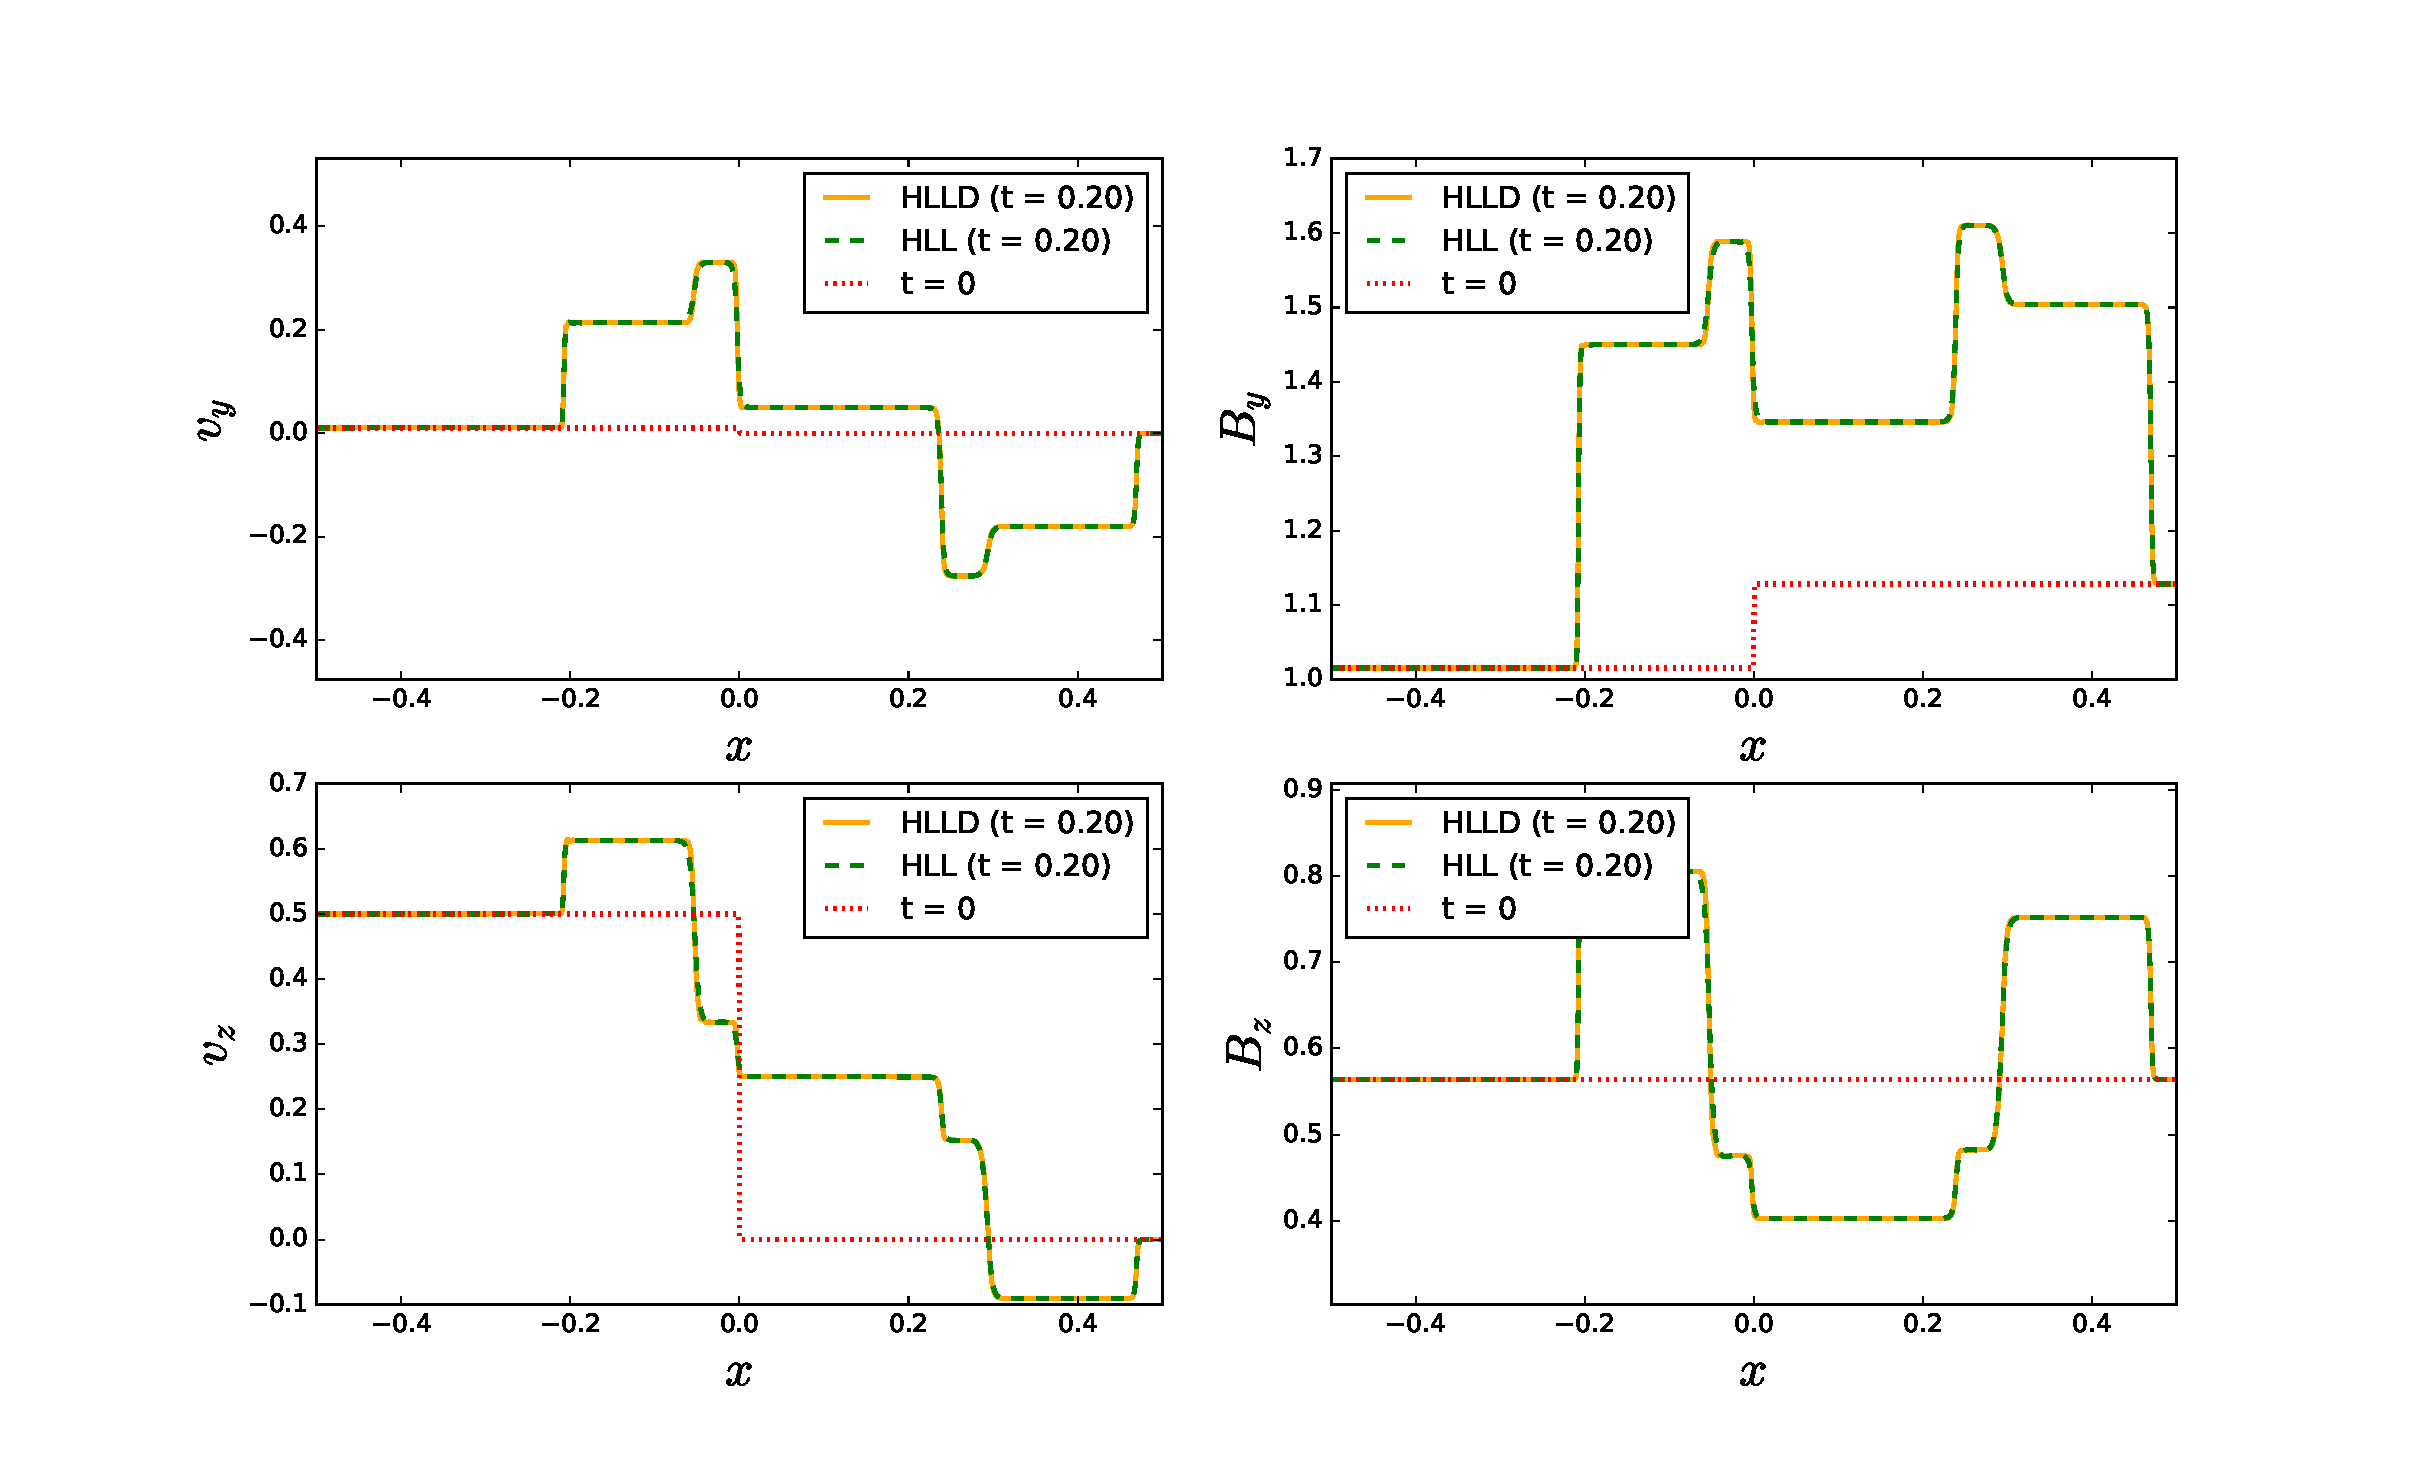
\includegraphics[width=1\textwidth]{DW2.eps}
	\end{minipage}%
\caption{Numerical solutions of Dai \& Woodward shock tube at time $t=0.2$ using HLLD and HLL 
schemes are plotted. The red dotted curves are the initial conditions of the shock tube.}
\label{fig: DW shock test}
\end{figure}

\clearpage

\subsection{Brio \& Wu test}
A standard test for MHD code is Brio \& Wu test. Following Stone et al. (2008) \cite{stone2008athena}, the Brio \& Wu problem is solved within the region 
$x \in [0,1]$ with 800 cells  and the initial set-up (at $t=0$) is given by 
\begin{align}
&(\rho,\ P,\ v_x,\ v_y,\ v_z,\ B_y,\ B_z) = (1.0, 1.0, 0, 0, 0, 1.0, 0) \quad
\text{for } x<0.5 \ , \\
&(\rho,\ P,\ v_x,\ v_y,\ v_z,\ B_y,\ B_z) = (0.125, 0.1, 0, 0, 0, -1.0,0) \quad
\text{for } x\geq0.5  \ , 
\end{align}
with $B_x = 0.75$ and $\gamma = 2.0$. The CFL number is set to be 0.3.

Fig. \ref{fig: BW shock test} illustrates the numerical solution to Brio \& Wu shock test 
at time $t=0.08$. 
Compared to the results in previous work (e.g. Stone et al \cite{stone2008athena} and 
Miyoshi \& Kusano \cite{miyoshi2005multi}), my MHD code captures all the features 
of the shocks and discontinuities. However, we should expect more obvious difference between 
the HLLD realization and the regular HLL realization. The HLLD scheme is supposed to 
have much higher resolution than the regular HLL scheme since more intermediate 
states are used in HLLD to accurately depict the fluxes through each interface. This may 
indicate that my HLLD code could be further promoted to a higher-accuracy version.
\begin{figure}[ht]
	\centering
	\begin{minipage}[c]{0.9\textwidth}
		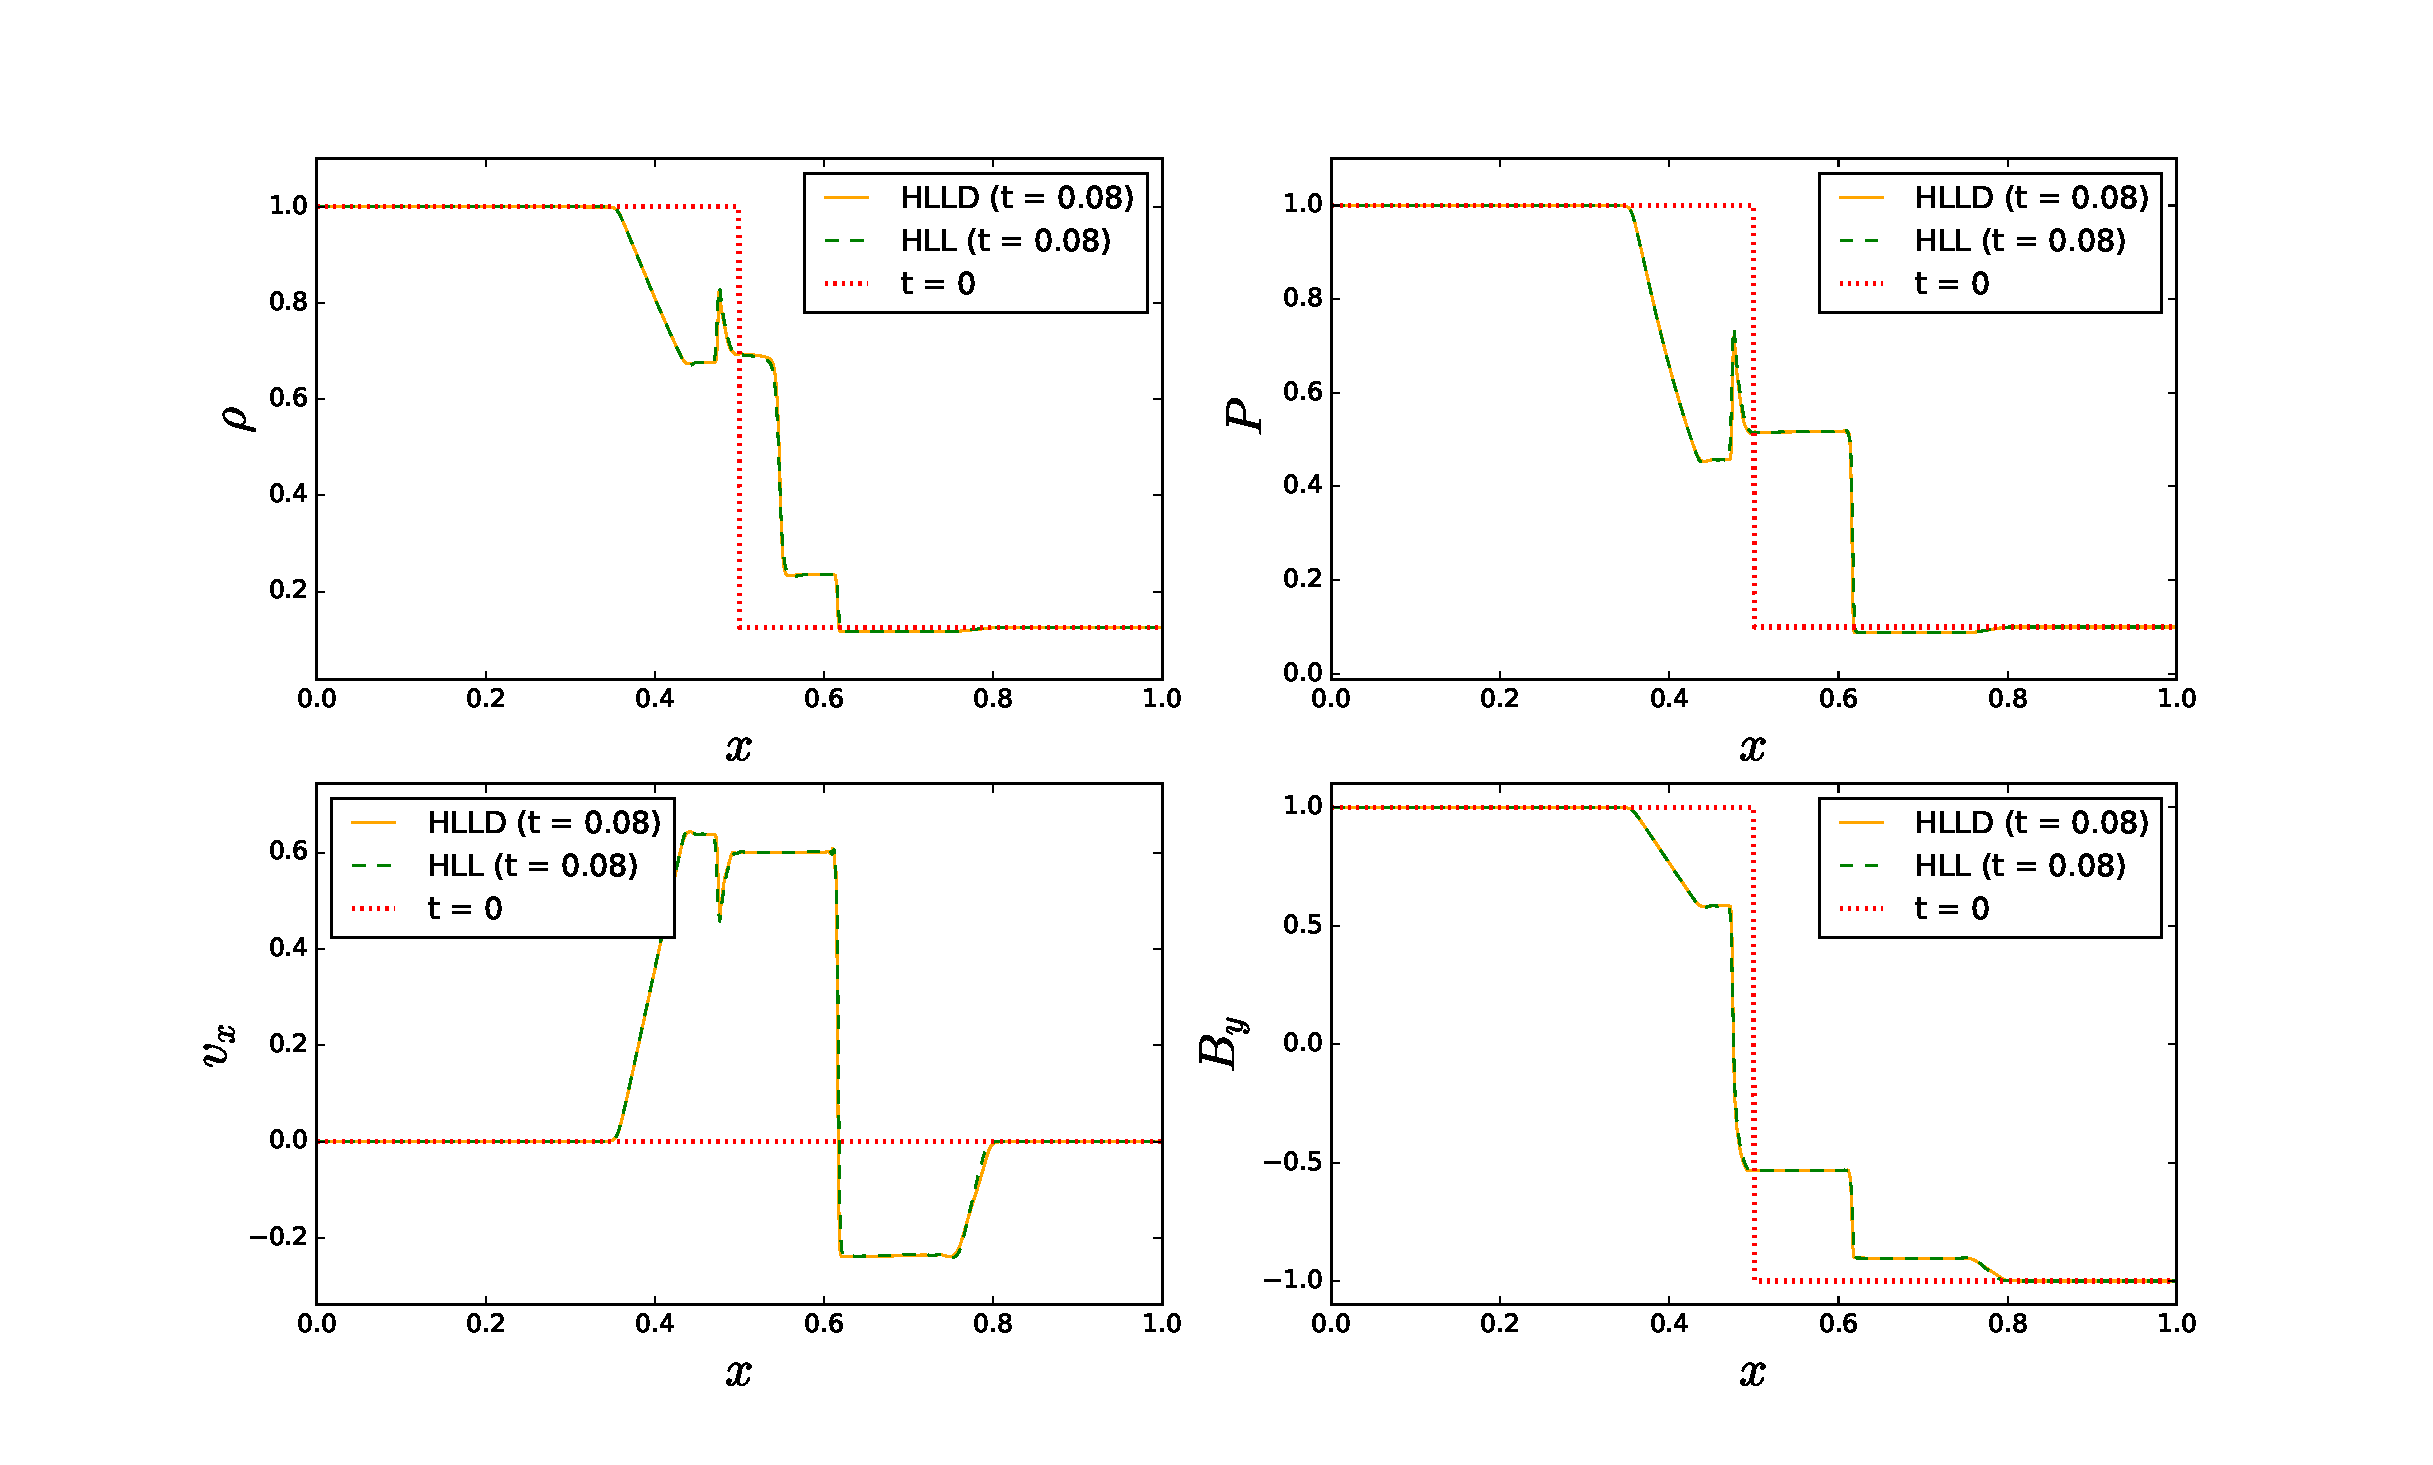
\includegraphics[width=1\textwidth]{BW1.eps}
	\end{minipage}
	\begin{minipage}[c]{0.9\textwidth}
		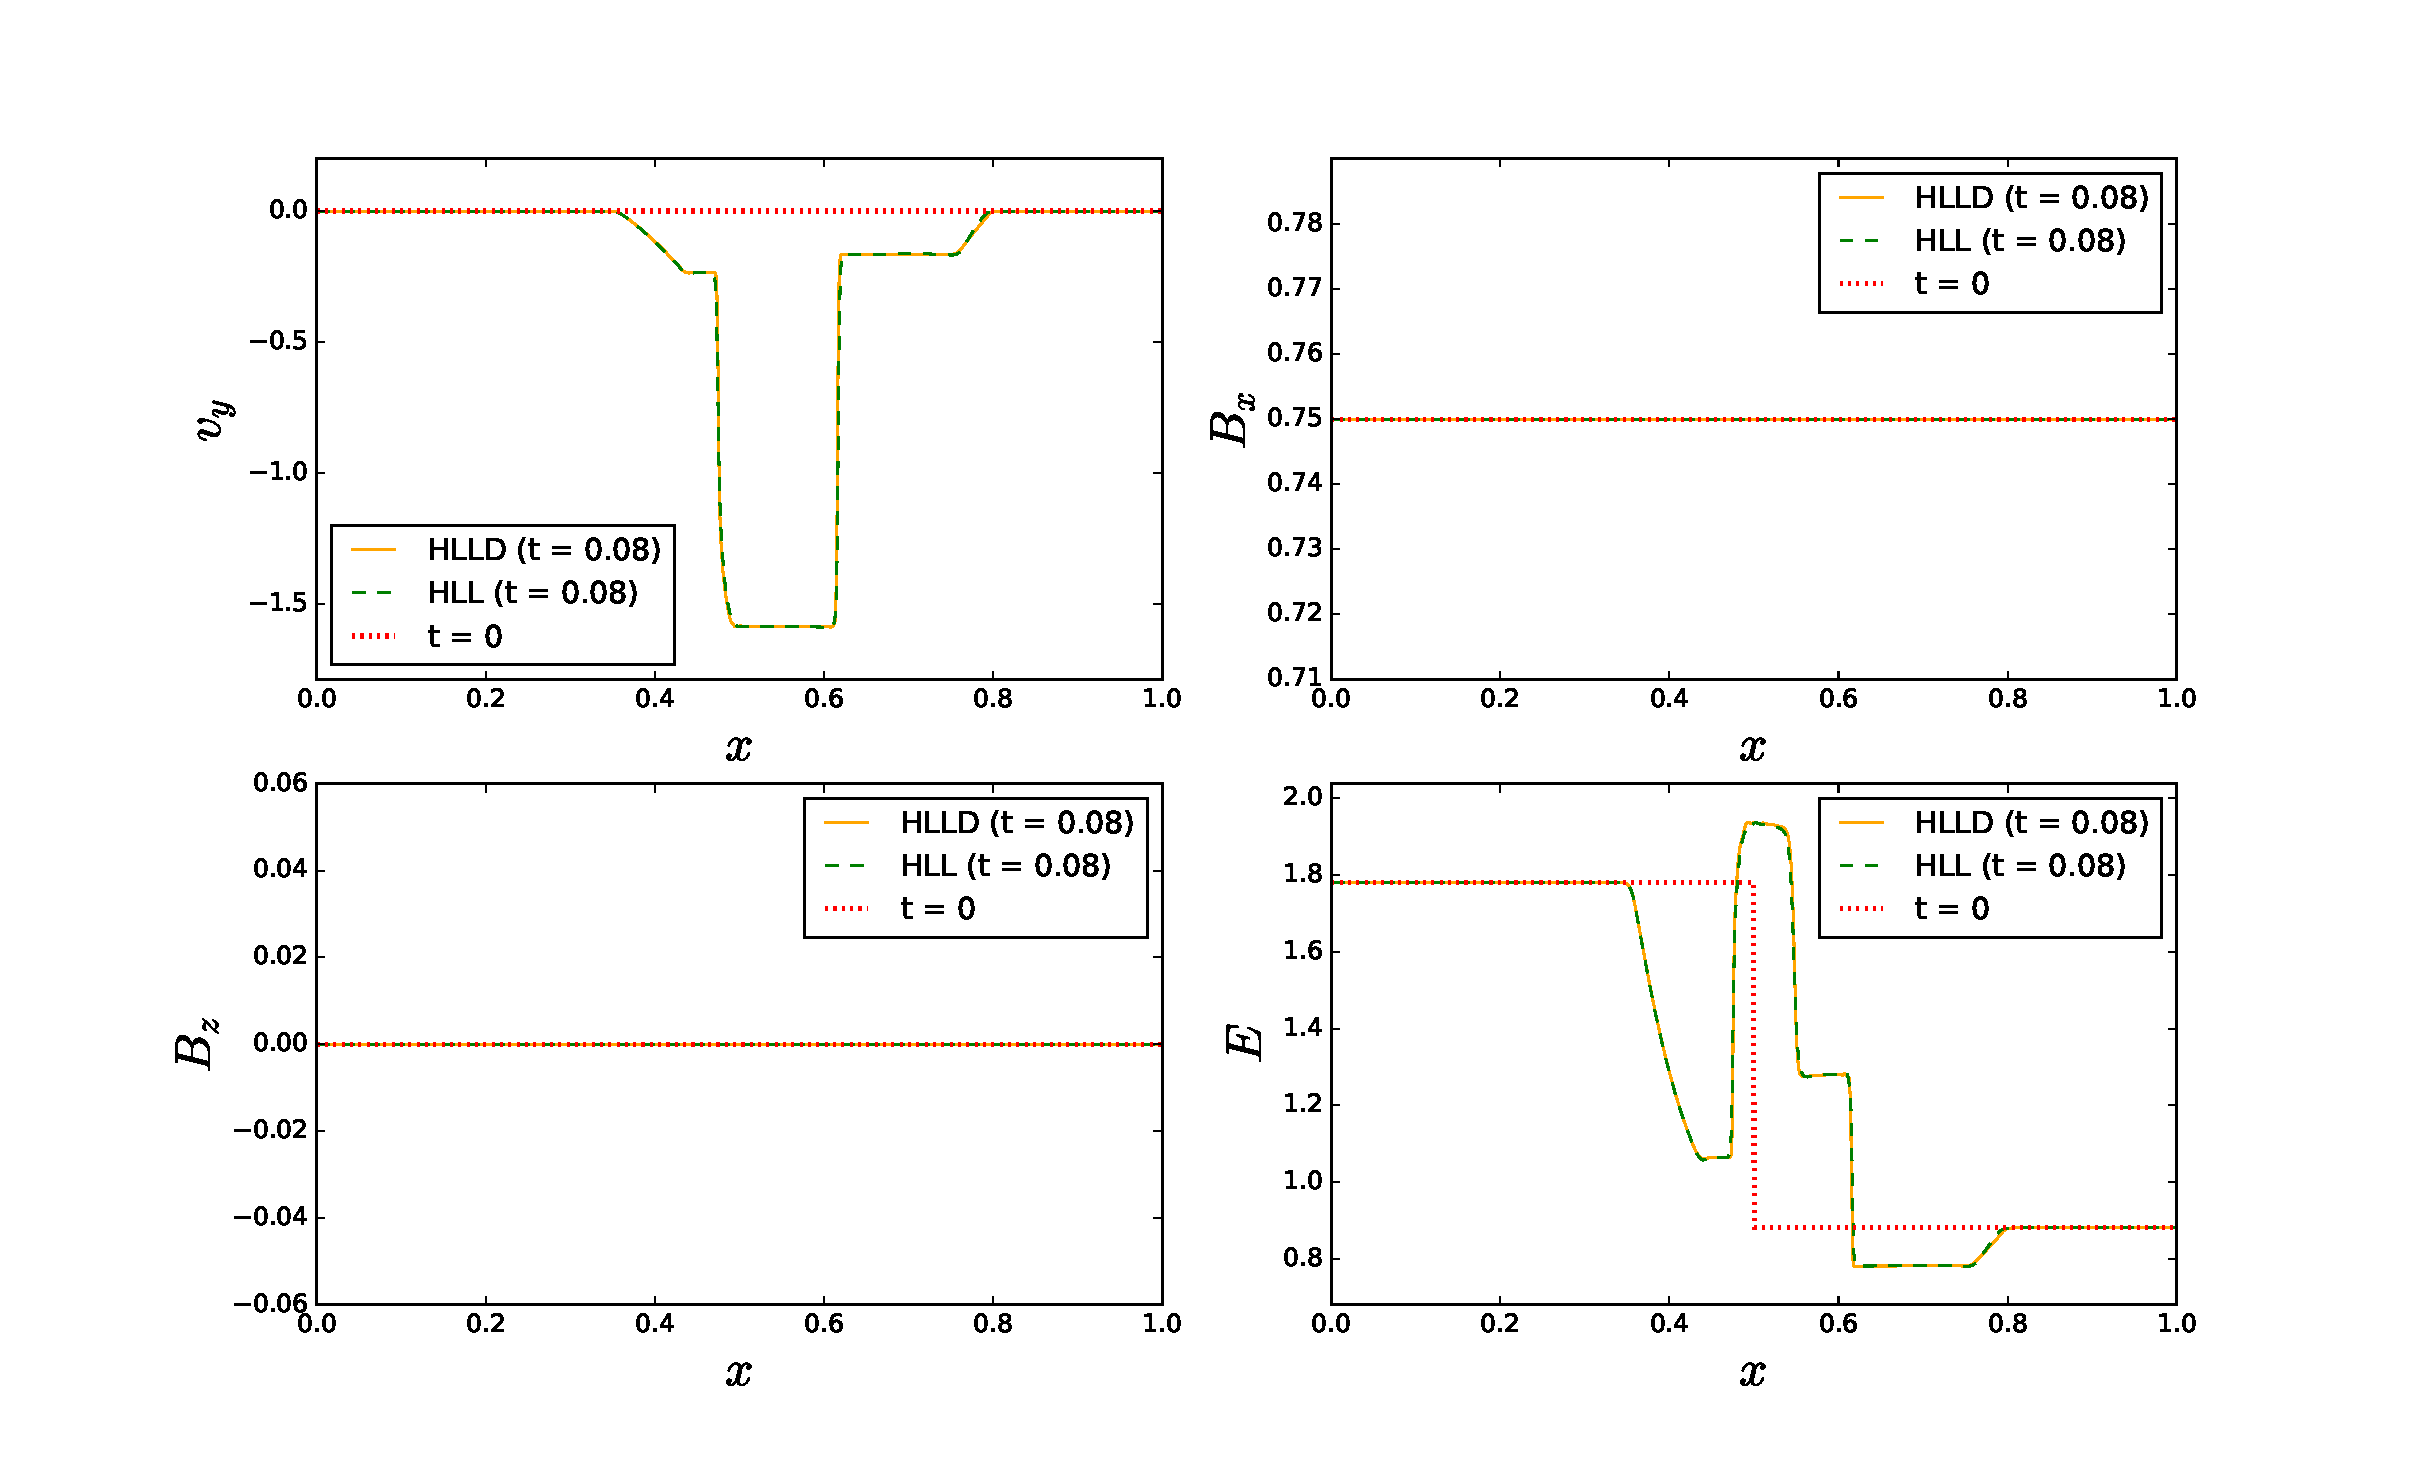
\includegraphics[width=1\textwidth]{BW2.eps}
	\end{minipage}%
\caption{Numerical solutions of Brio \& Wu shock test at time $t=0.08$ using HLLD and HLL 
schemes are plotted. The red dotted curves are the initial conditions of the shock tube.}
\label{fig: BW shock test}
\end{figure}

\subsection{Alfv\'en Wave realization}
To realize a sinusoidal Alfv\'en wave, we apply PLM + HLLD scheme to 
study the MHD system with $\gamma = 5/3$ 
using 800 cells within $x\in[-1,1]$ and set a periodic boundary for the system. 
The CFL number is chosen to be 0.6.
The initial conditions for the system is given by 
\begin{align}
&(\rho,\ P,\ v_x) = (1.0,1.0,0) \ , \\
&(\ v_y,\ v_z) = (0.1 \sin[2 \pi x  \cos(\alpha)], 0.1 \cos[2 \pi x  \cos(\alpha)]) \ , 
\label{eq: transverse velocity}\\
&(B_y,\ B_z) = (0.1 \sin[2 \pi x  \cos(\alpha)], 0.1 \cos[2 \pi x  \cos(\alpha)]) \ , 
\label{eq: transverse magnetic field}
\end{align}
with $\alpha=0$, $B_x=1.0$.
The wave speed of Alfv\'en wave can be immediately calculated as 
$c_a = \frac{|B_x|}{\sqrt{\rho}} = 1.0$. By equation (\ref{eq: transverse velocity}) 
and (\ref{eq: transverse magnetic field}), we obtain the wavelength is $\lambda_a=1$,
therefore the period of the Alfv\'en wave is simply $T_a = \lambda_a / c_a =1$.

Fig. \ref{fig: AW} displays the evolution of the system. The wave shown is a transverse wave 
with the polarization in $y-z$ plane and the transmission in $x$ direction.
The period of the wave constructed is consistent with the theoretical expectation of the 
Alfv\'en wave under the given initial conditions.

\begin{figure}[ht]
	\centering
	\begin{minipage}[c]{0.9\textwidth}
		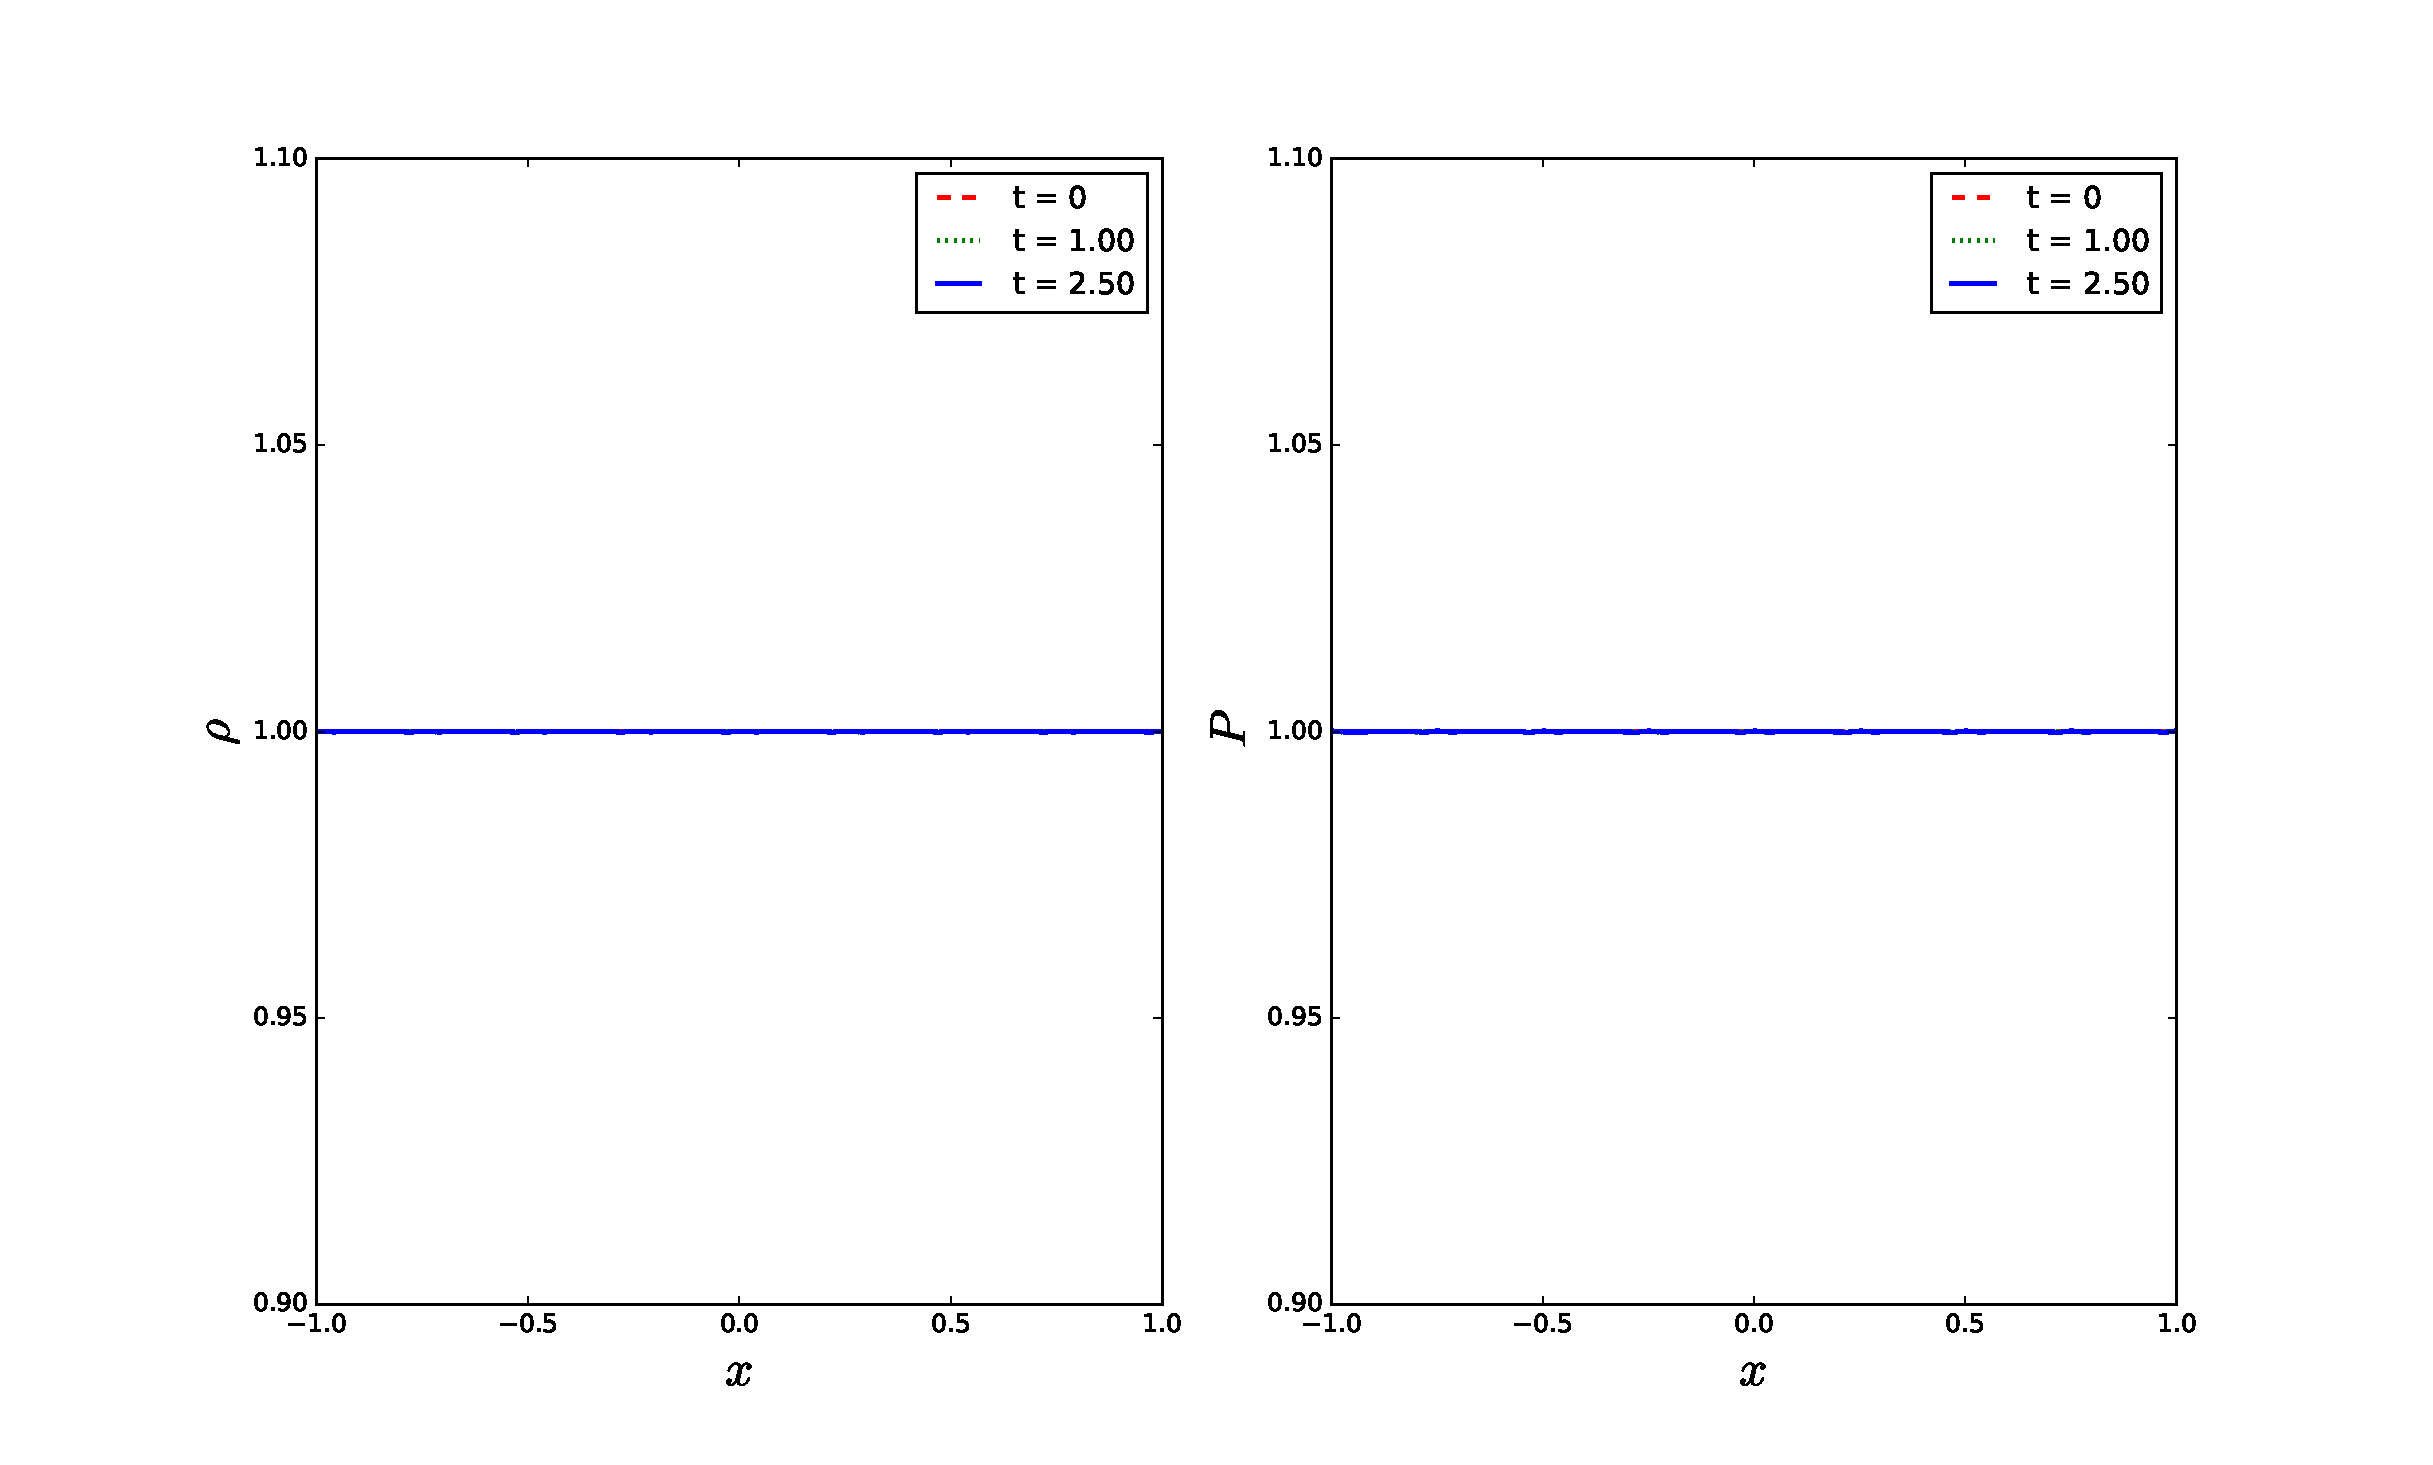
\includegraphics[width=1\textwidth]{AW1.eps}
	\end{minipage}
	\begin{minipage}[c]{0.9\textwidth}
		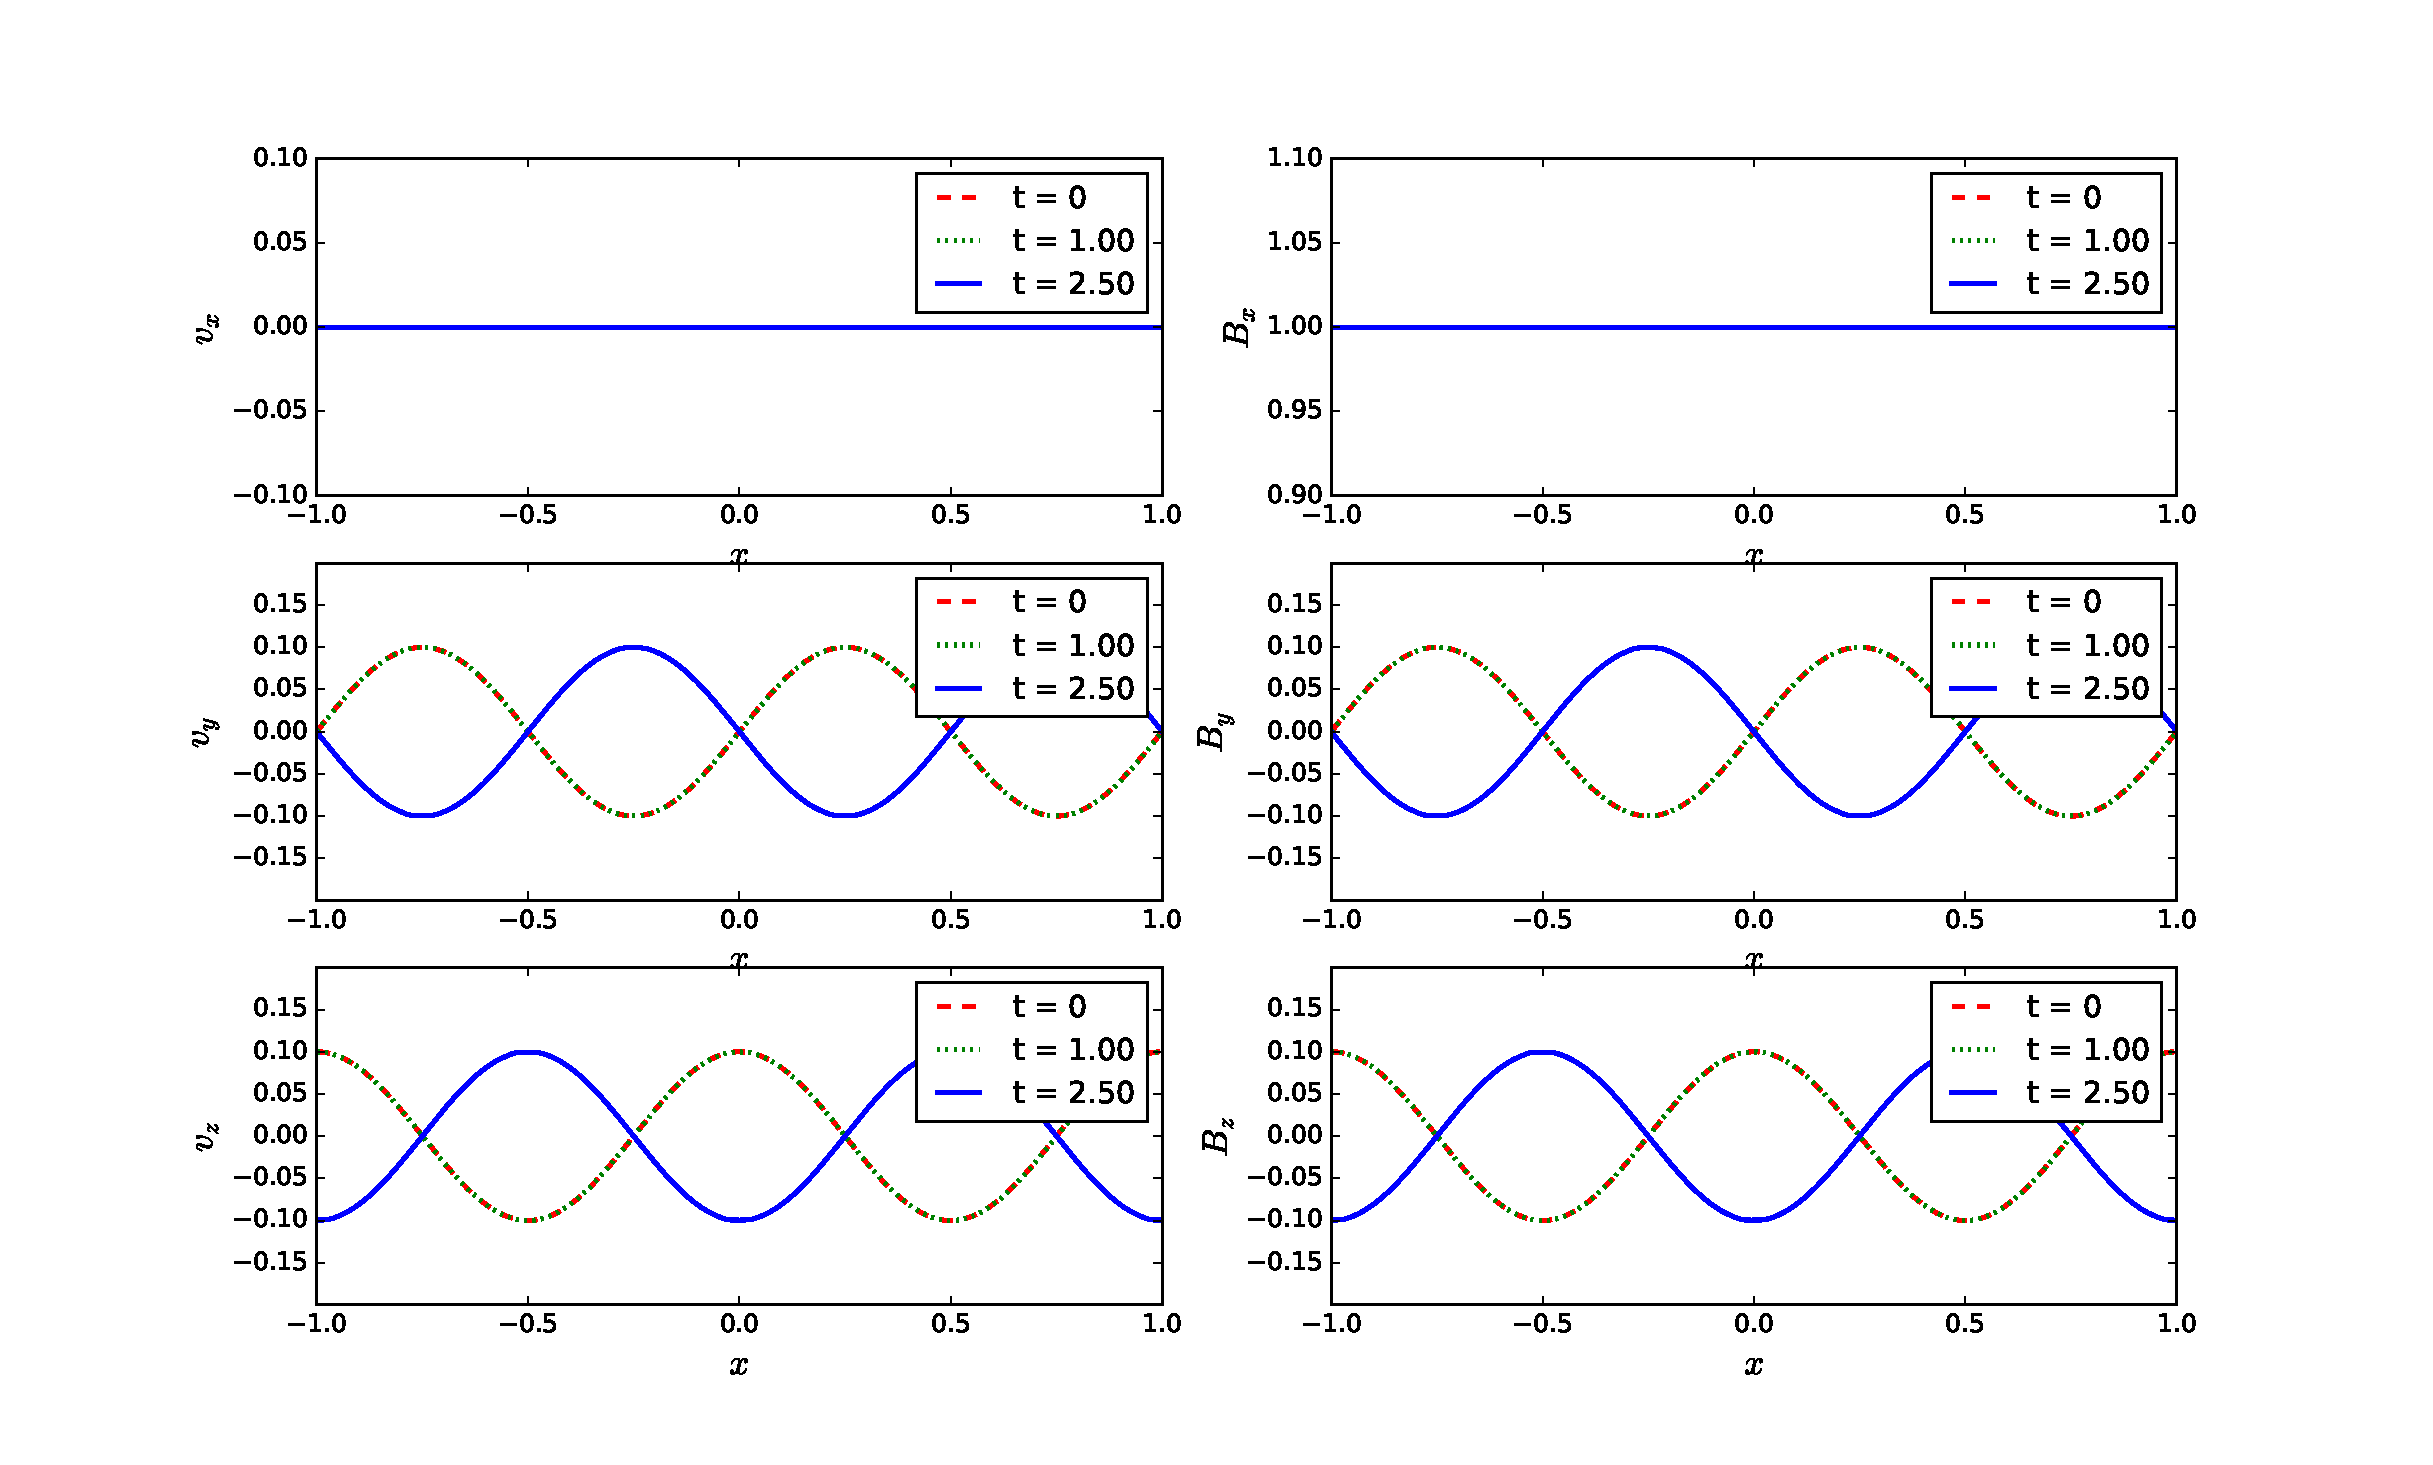
\includegraphics[width=1\textwidth]{AW2.eps}
	\end{minipage}%
\caption{Numerical construction of the Alfv\'en wave using HLLD 
scheme is plotted. The red dashed curves are the initial conditions.}
\label{fig: AW}
\end{figure}

\clearpage

\subsection{Fast Switch-on (FS) shock}
Falle et al. (1998) \cite{falle1998} proposed that the most rational procedure is to test MHD 
code with a complete set of pure waves rather than compound waves like the shocks in 
Brio \& Wu test.
A first example of these pure wave tests is fast switch-on (FS) shock. The FS shock is 
constructed using PLM + HLLD in the region $x\in[-0.5,3]$ with 400 cells, $\gamma=5/3$ and CFL number 0.3. 
The initial condition is given by 
\begin{align}
	&(\rho,\ P,\ v_x,\ v_y,\ v_z,\ B_y,\ B_z) = (3, 16.33, -0.732, -1.333, 0, 2.309, 1) \quad
	\text{for the left half region}  \ , \\
	&(\rho,\ P,\ v_x,\ v_y,\ v_z,\ B_y,\ B_z) = (1,1,-4.196,0,0,0,0) \quad
	\text{for the right half region}  \ , 
\end{align}
with $B_x = 3$ everywhere. 

Fig. \ref{fig: FS test} illustrates the FS shock evolution. Some small-amplitude waves emerge in 
Fig. \ref{fig: FS test}, which travel away from the shock. It is said that these are 
generated when the initially discontinuity
evolves into a steadily propagating shock with finite width.
\begin{figure}[ht]
	\centering
	\begin{minipage}[c]{0.9\textwidth}
		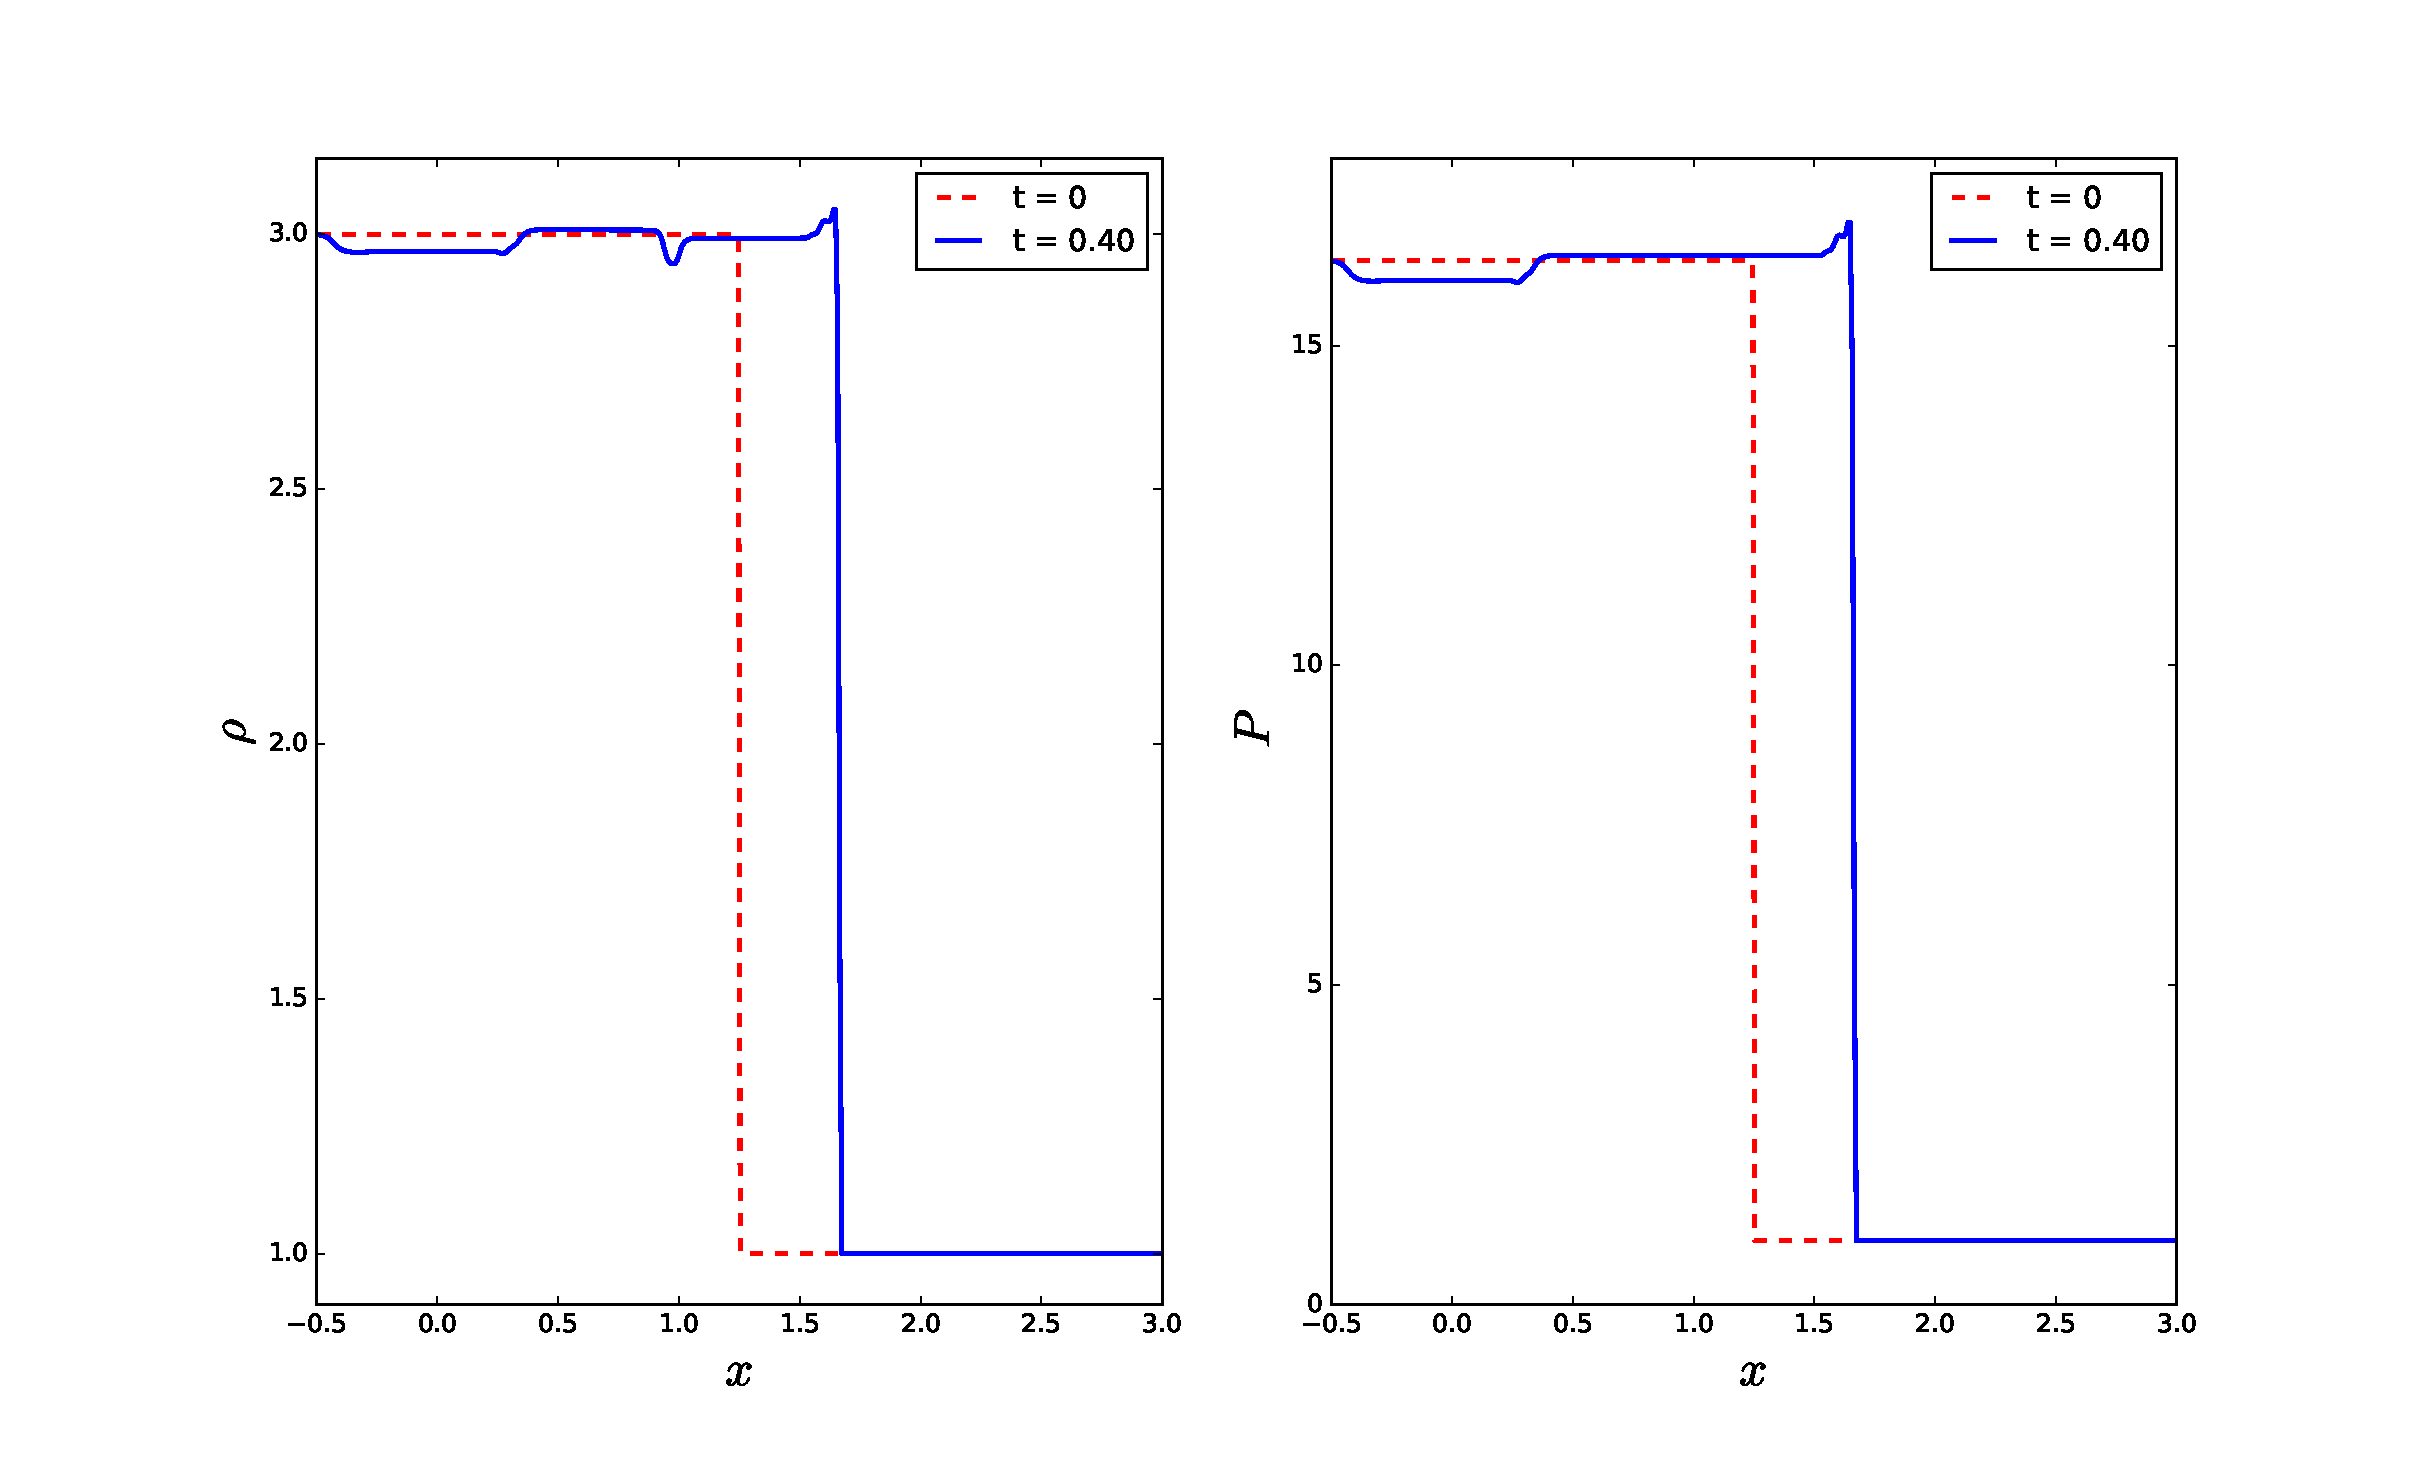
\includegraphics[width=1\textwidth]{FS1.eps}
	\end{minipage}
	\begin{minipage}[c]{0.9\textwidth}
		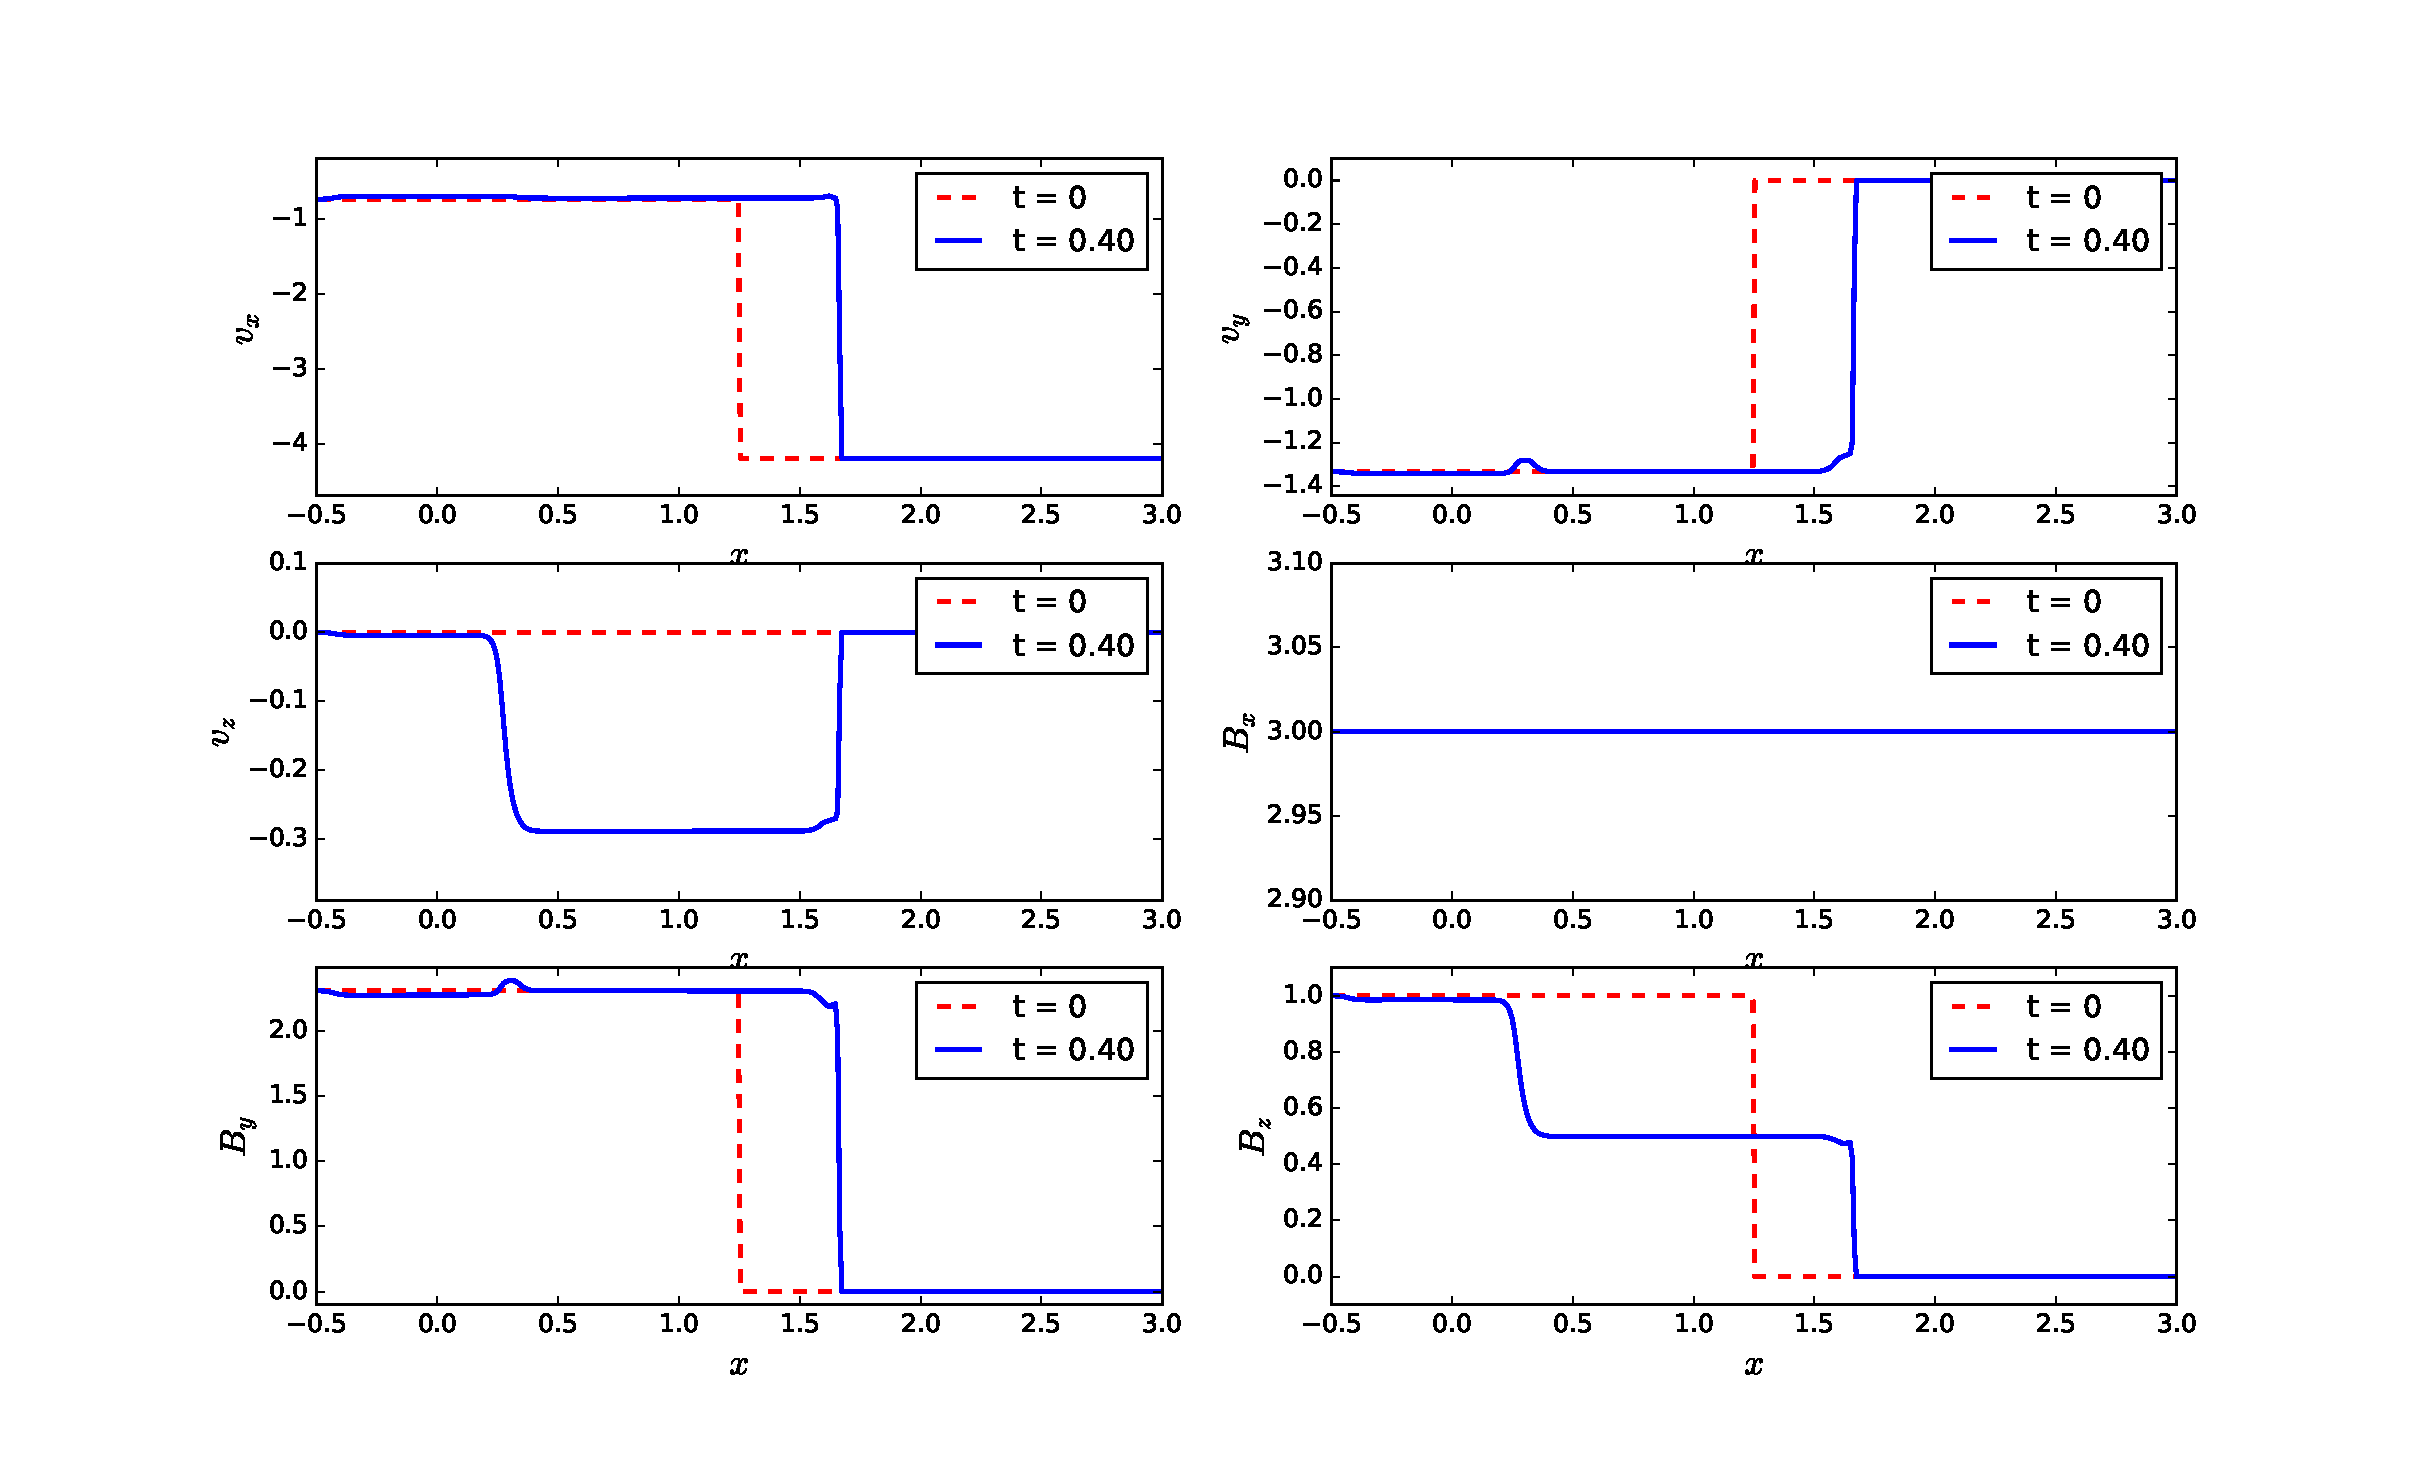
\includegraphics[width=1\textwidth]{FS2.eps}
	\end{minipage}%
\caption{The evolution of FS shock from $t=0$ to $t=0.4$ is plotted. 
The red dashed curves are the initial conditions of the shock tube.}
\label{fig: FS test}
\end{figure}


\subsection{Slow Switch-off (SS) shock}
Similarly, Falle et al. proposed the Slow Switch-off (SS) shock test in contrast to FS shock.
The SS shock is constructed using PLM + HLLD in the region $x\in[-0.5,1.5]$ with 400 cells, $\gamma=5/3$ and 
CFL number 0.3.
The initial condition is given by 
\begin{align}
	&(\rho,\ P,\ v_x,\ v_y,\ v_z,\ B_y,\ B_z) = (1.368,1.769,0.269,1.0,0,0,0) \quad
	\text{for the left half region}  \ , \\
	&(\rho,\ P,\ v_x,\ v_y,\ v_z,\ B_y,\ B_z) = (1,1,0,0,0,1,0) \quad
	\text{for the right half region}  \ , 
\end{align}
with $B_x = 1$ everywhere. 
Fig. \ref{fig: SS test} illustrates the SS shock evolution.
\begin{figure}[ht]
	\centering
	\begin{minipage}[c]{0.9\textwidth}
		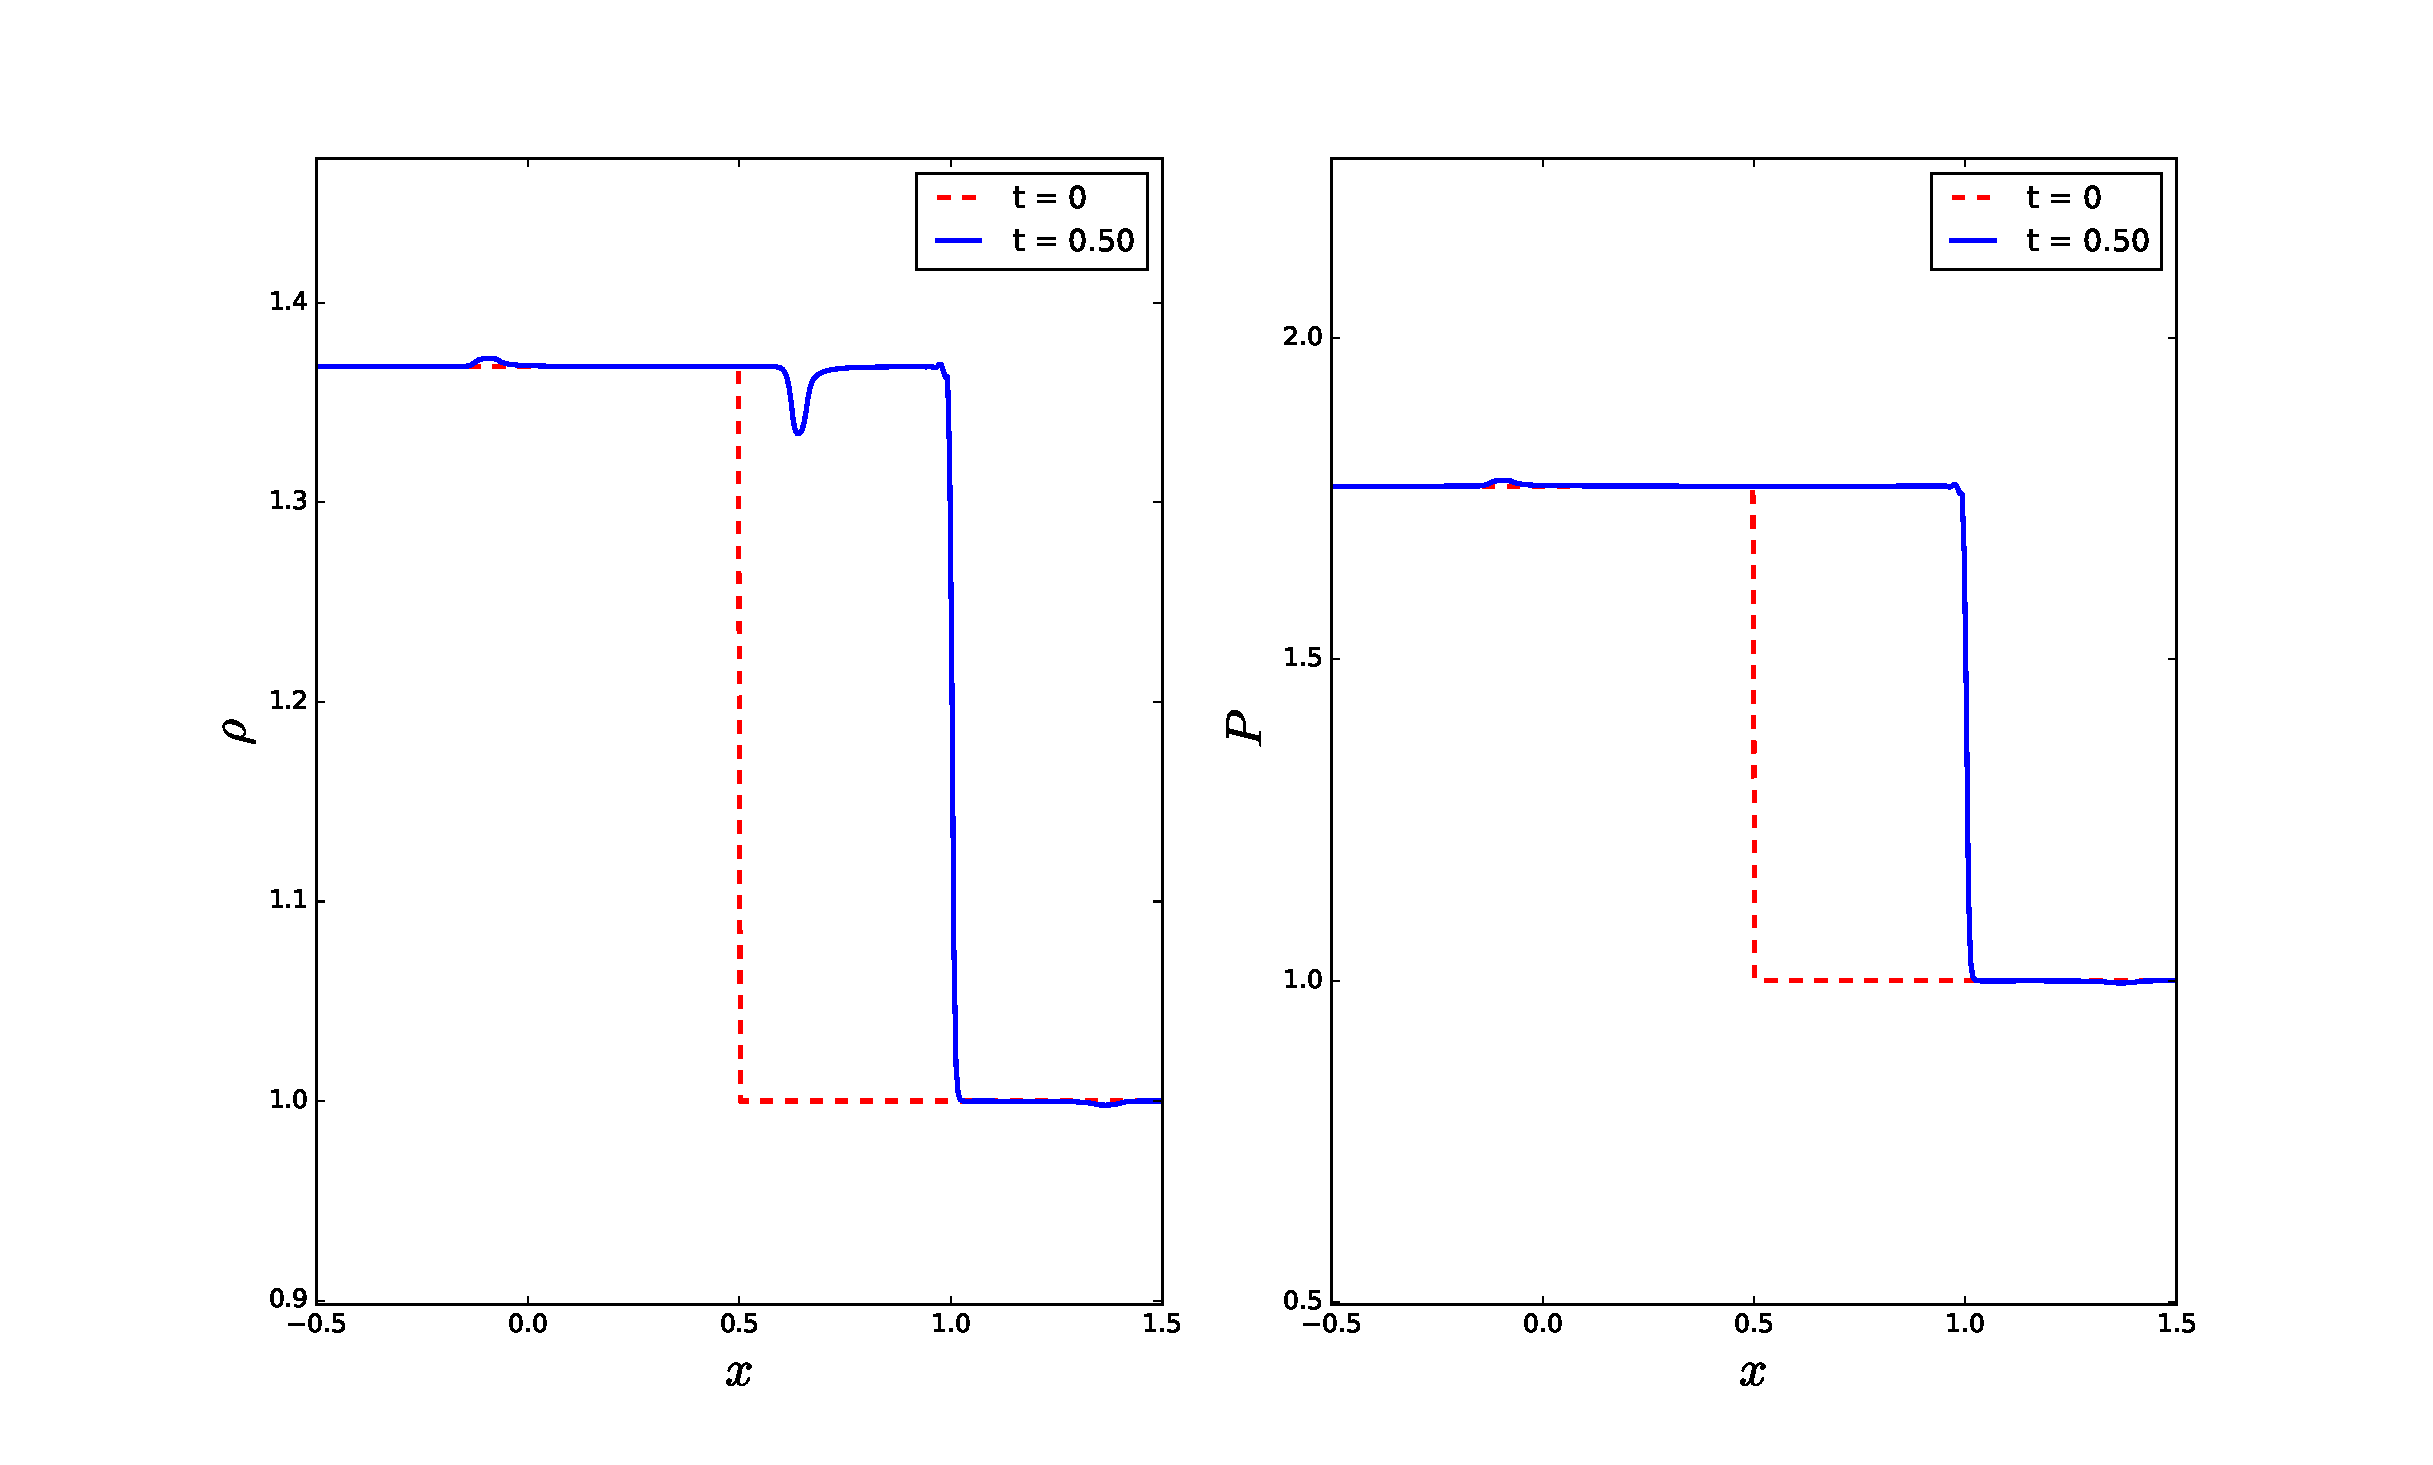
\includegraphics[width=1\textwidth]{SS1.eps}
	\end{minipage}
	\begin{minipage}[c]{0.9\textwidth}
		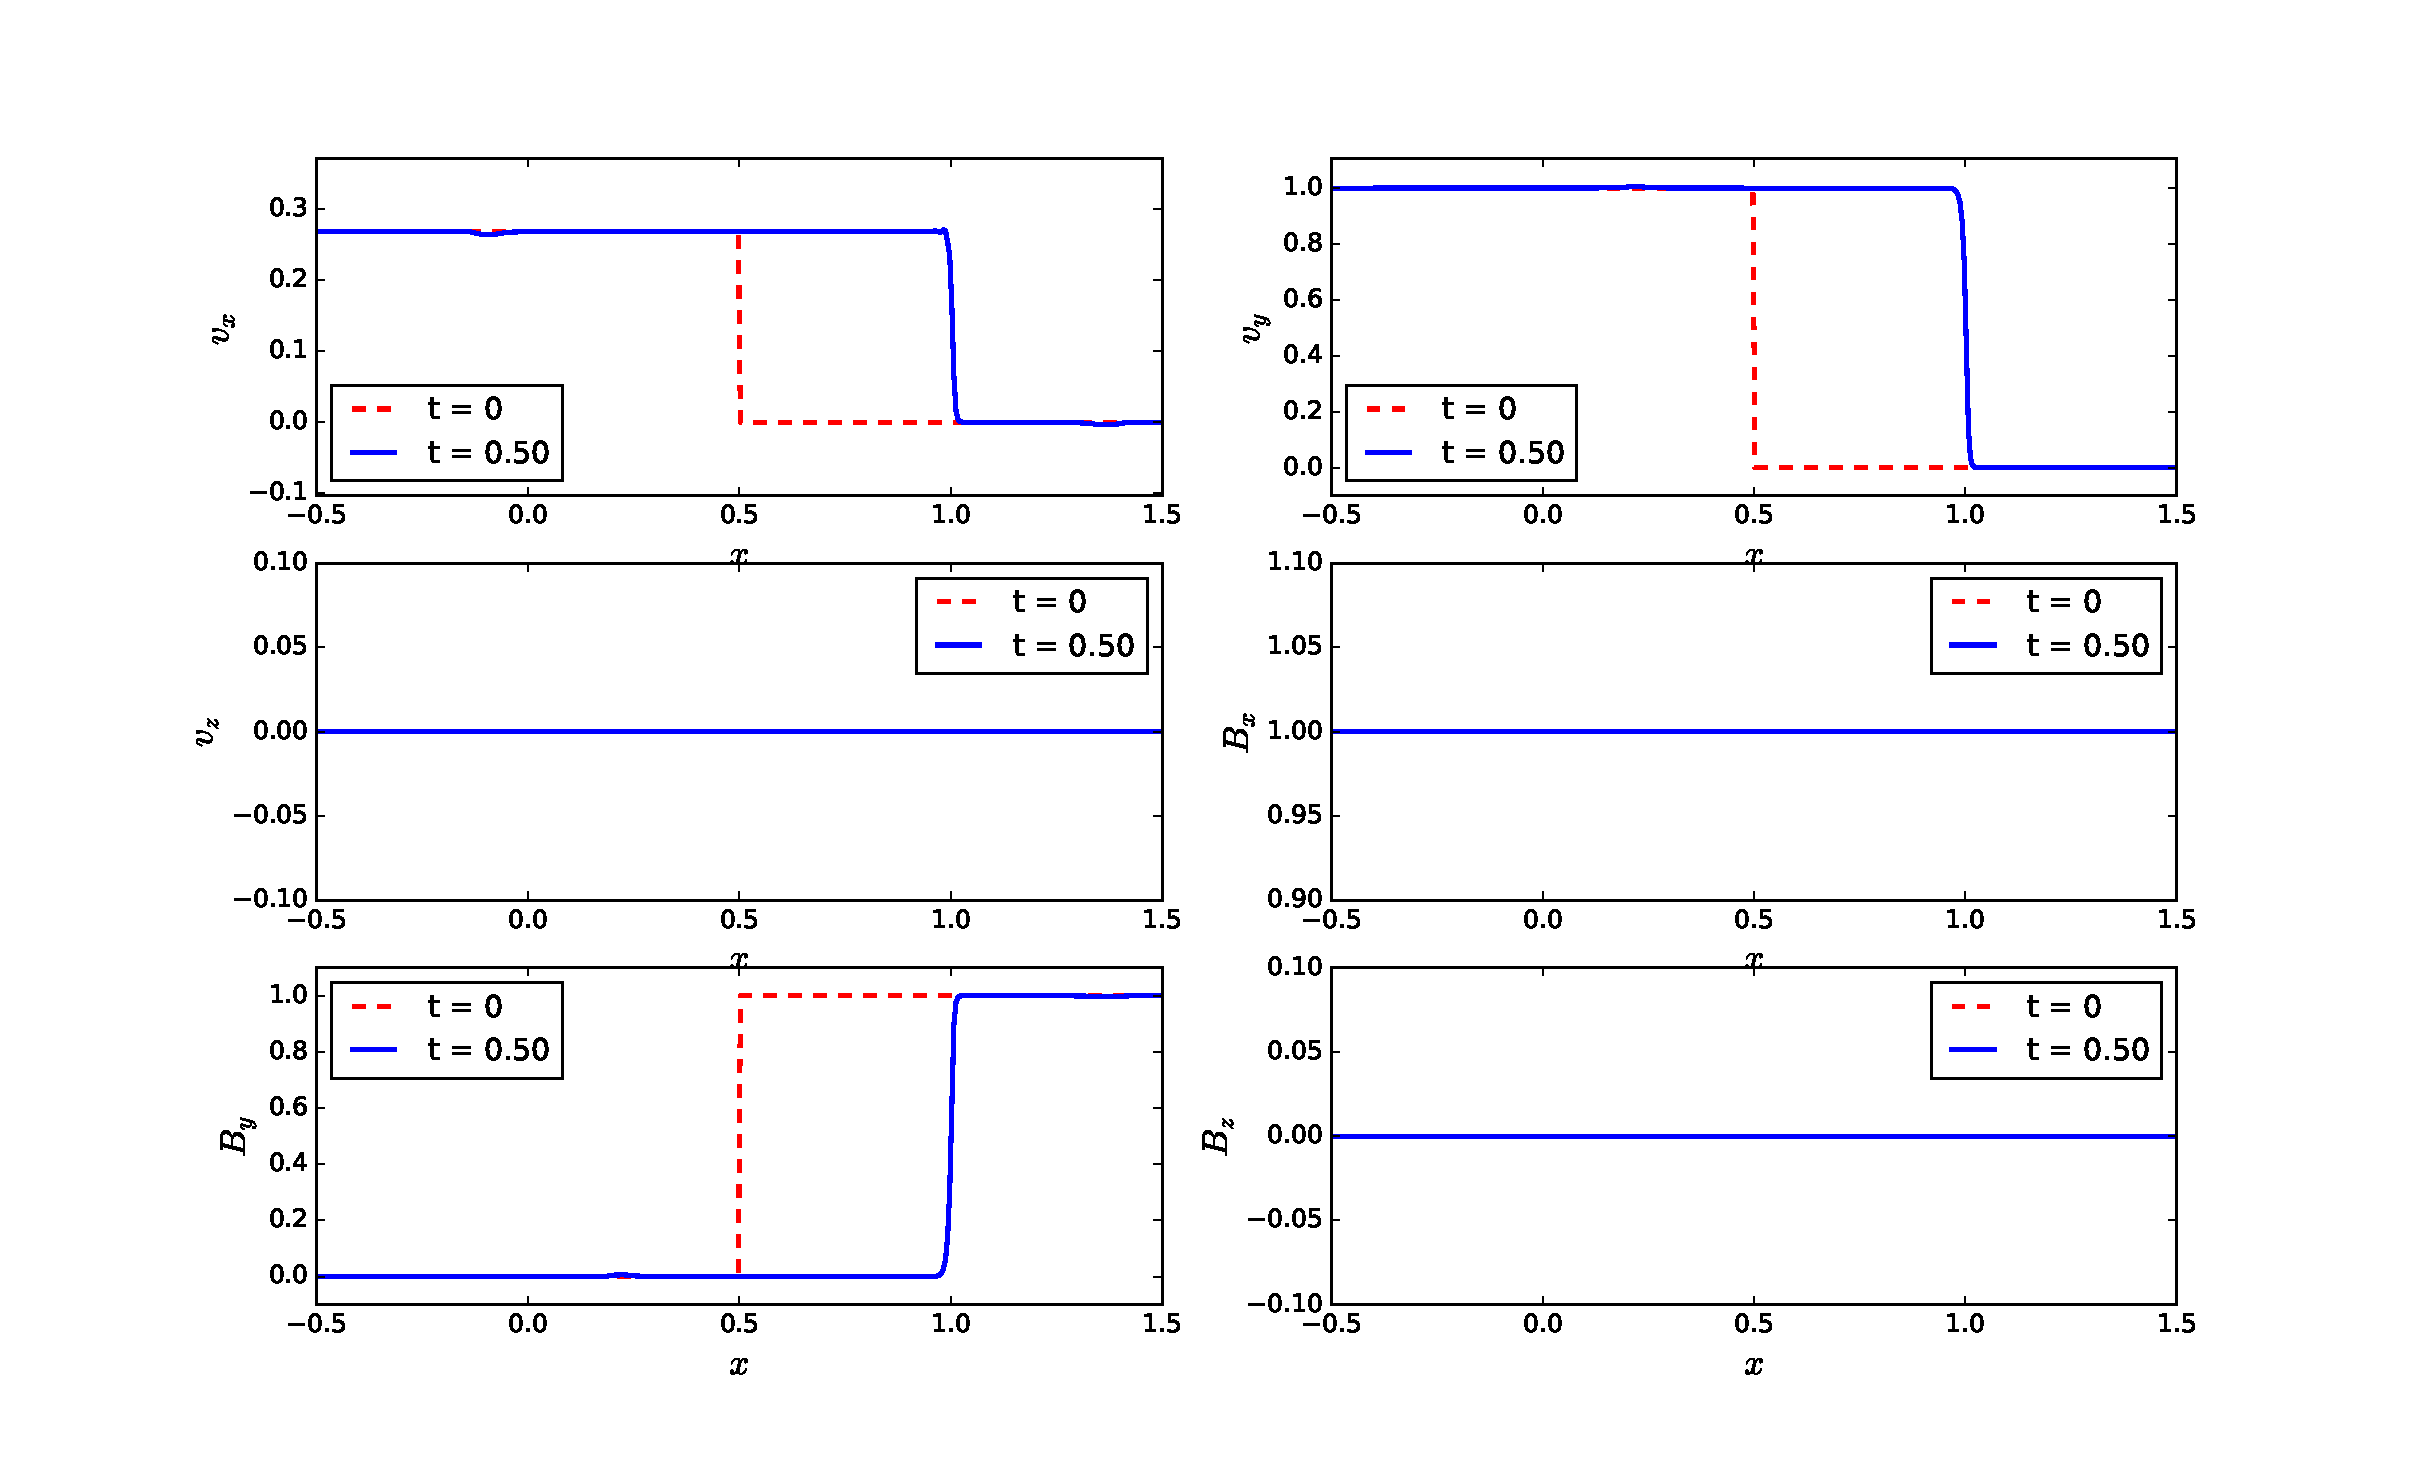
\includegraphics[width=1\textwidth]{SS2.eps}
	\end{minipage}%
\caption{The evolution of SS shock from $t=0$ to $t=0.5$ is plotted. 
The red dashed curves are the initial conditions of the shock tube.}
\label{fig: SS test}
\end{figure}

\subsection{Fast switch-off Rarefaction (FR) wave}
Falle et al.\cite{falle1998} also proposed a test in which the initial discontinuity evolves into
a fast rarefaction (FR) wave.
The FR wave is constructed using PLM + HLLD in the region $x\in[-0.5,1.5]$ with 400 cells, 
$\gamma=5/3$ and CFL number 0.3.
The initial condition is given by 
\begin{align}
	&(\rho,\ P,\ v_x,\ v_y,\ v_z,\ B_y,\ B_z) = (1,2,0,0,0,3,0) \quad
	\text{for the left half region}  \ , \\
	&(\rho,\ P,\ v_x,\ v_y,\ v_z,\ B_y,\ B_z) = (0.2641,0.2175,3.6,-2.551,0,0,0) \quad
	\text{for the right half region}  \ , 
\end{align}
with $B_x = 1$ everywhere. 
Fig. \ref{fig: FR test} shows the FR wave evolution.
\begin{figure}[ht]
	\centering
	\begin{minipage}[c]{0.9\textwidth}
		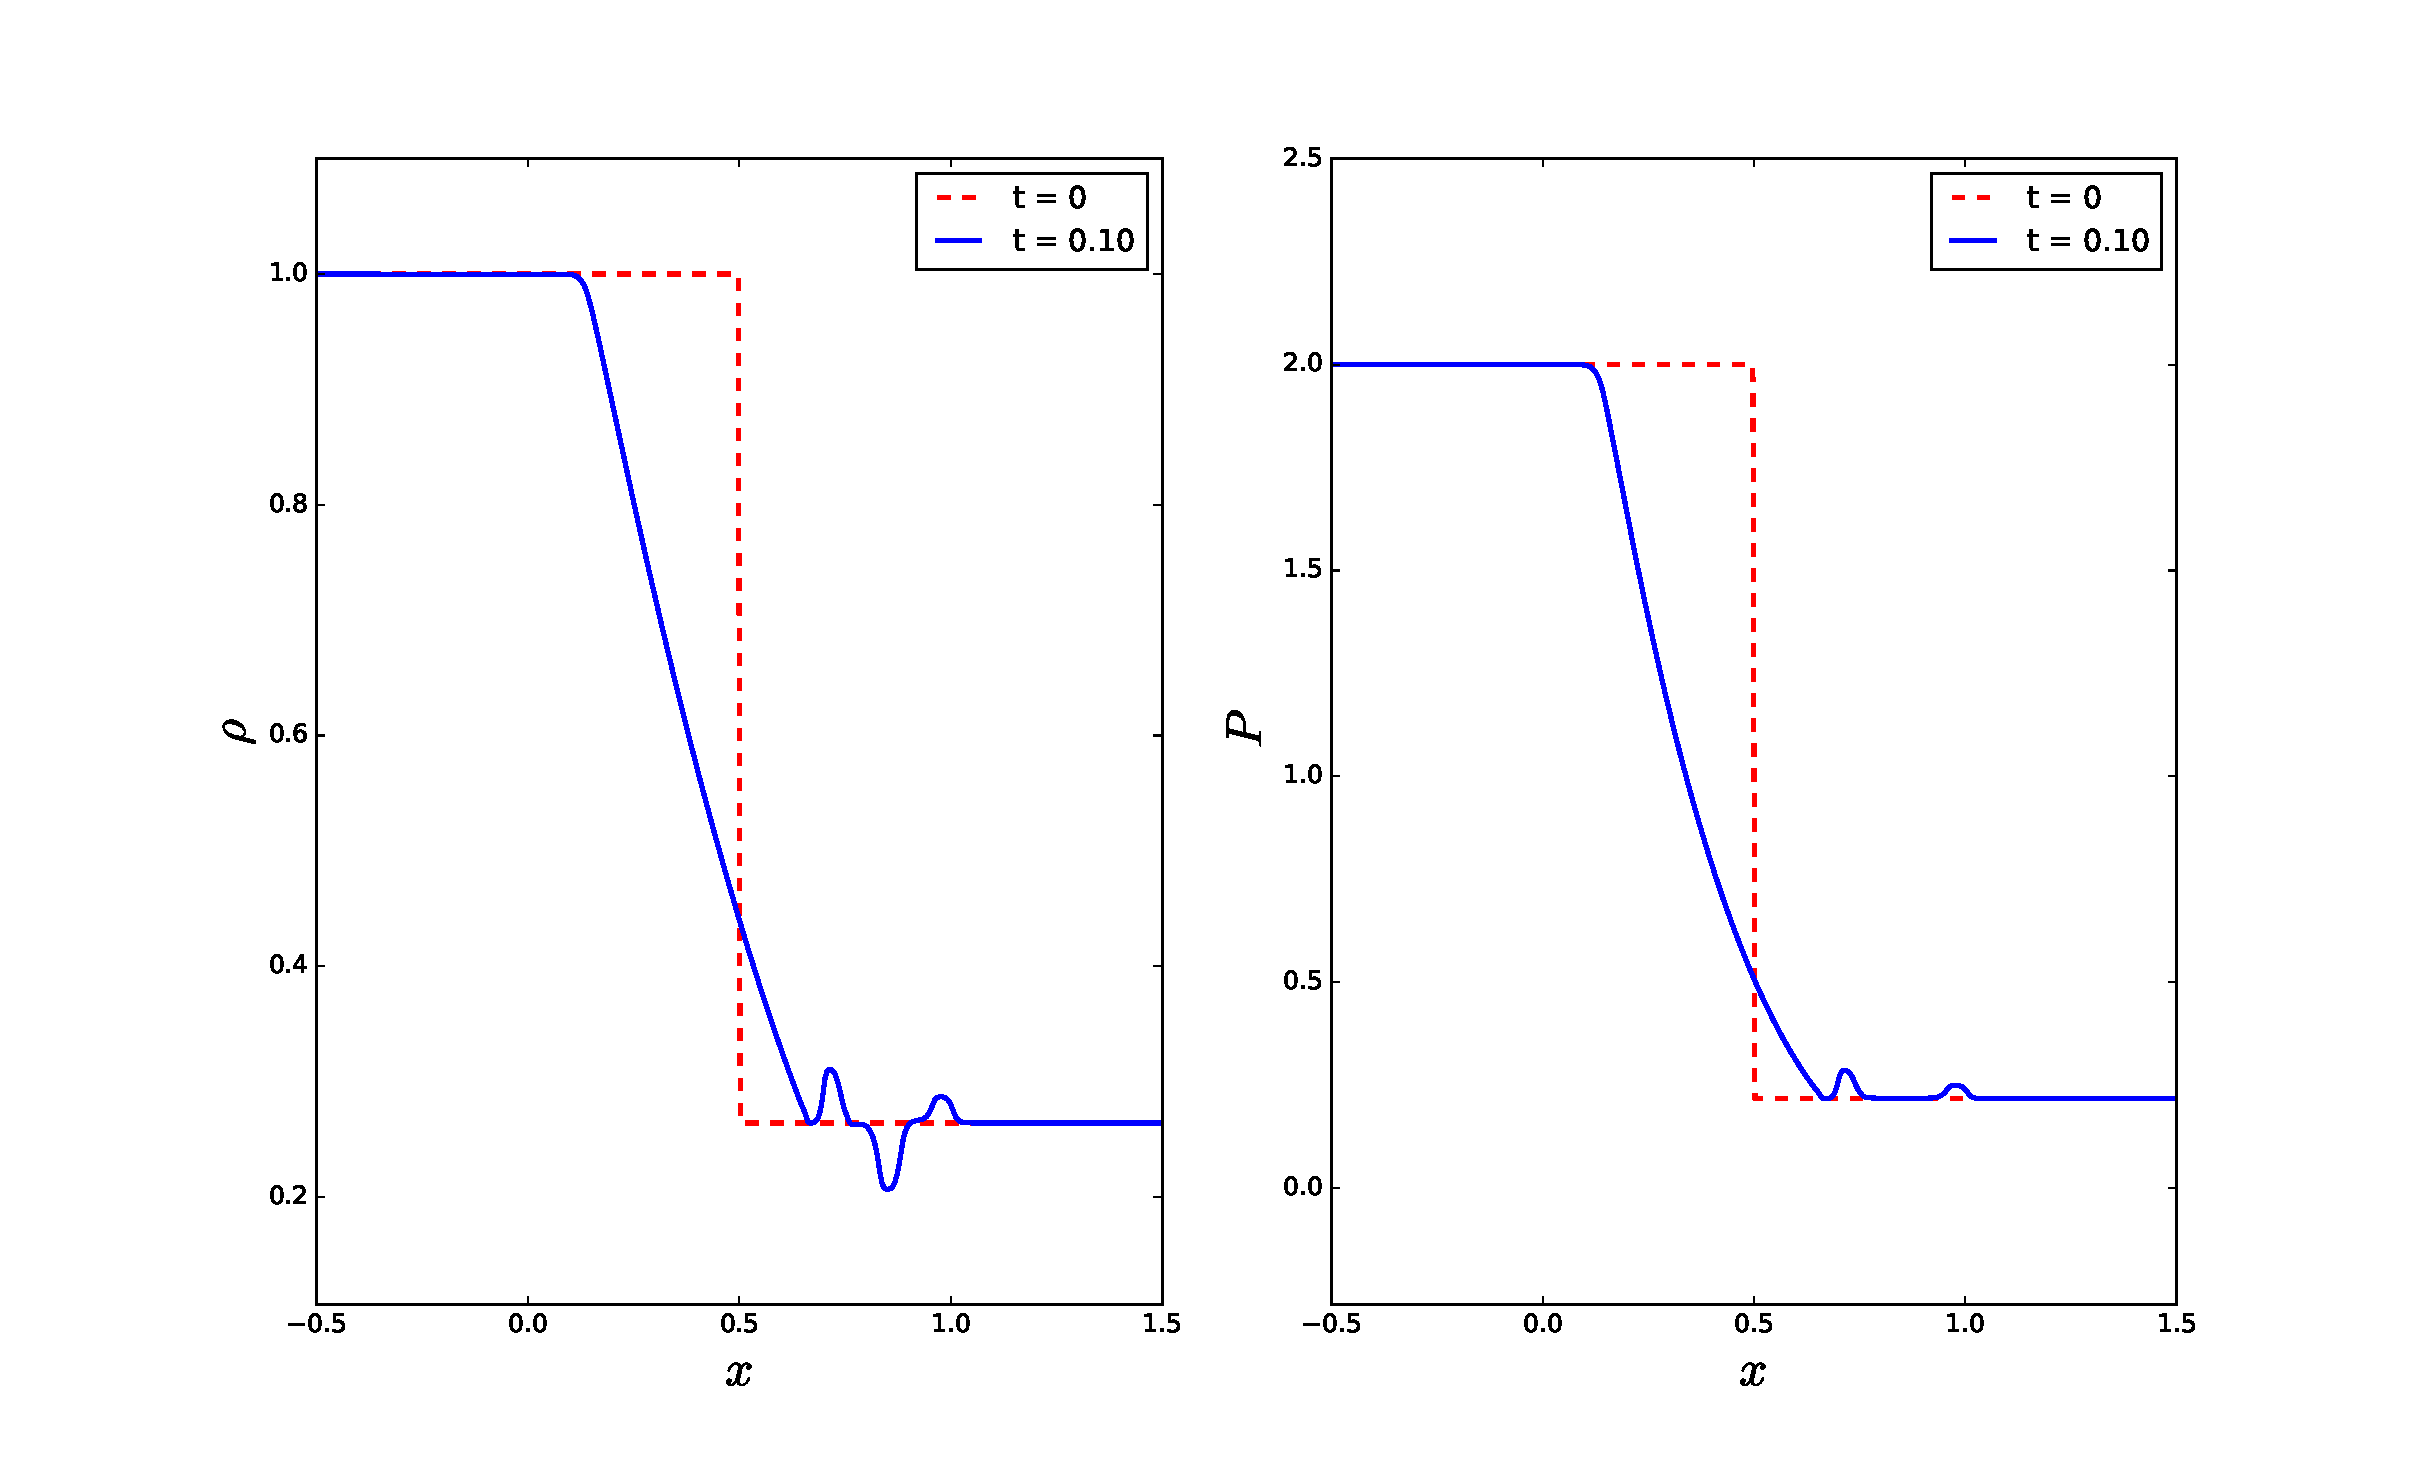
\includegraphics[width=1\textwidth]{FR1.eps}
	\end{minipage}
	\begin{minipage}[c]{0.9\textwidth}
		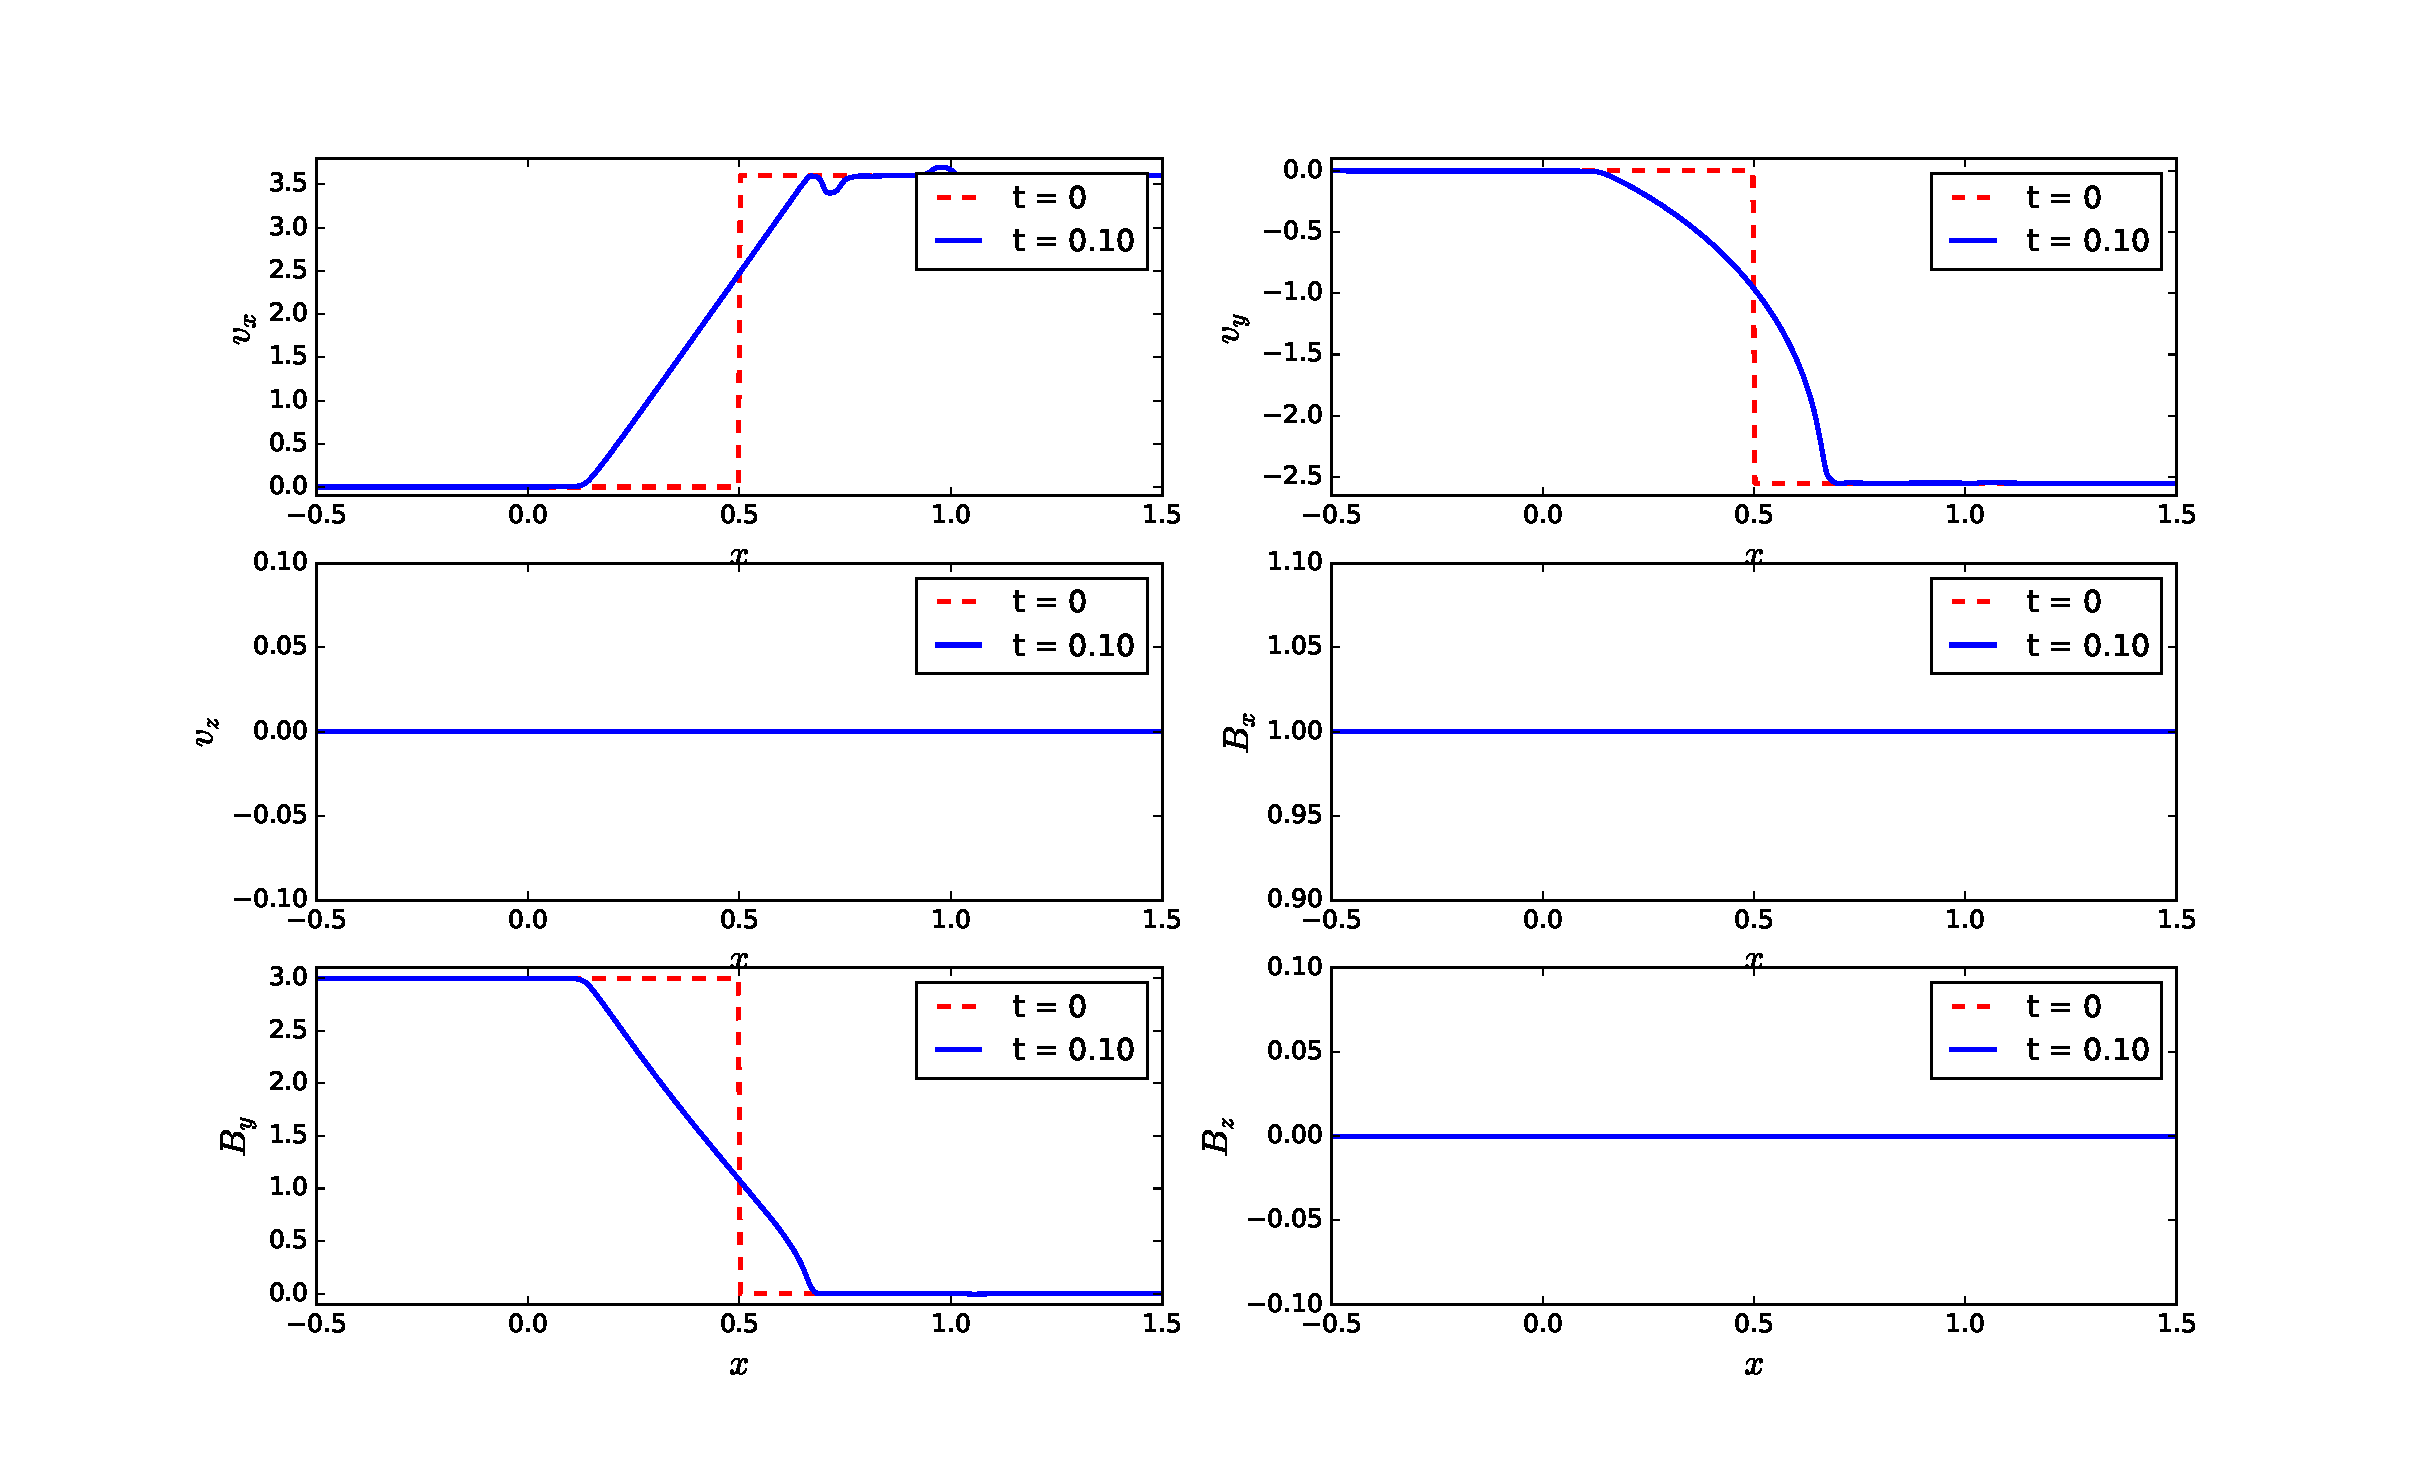
\includegraphics[width=1\textwidth]{FR2.eps}
	\end{minipage}%
\caption{The evolution of FR wave from $t=0$ to $t=0.1$ is plotted. 
The red dashed curves are the initial conditions.}
\label{fig: FR test}
\end{figure}

\subsection{Slow switch-on Rarefaction (SR) wave}
In contrast to FR waves, Falle et al.\cite{falle1998} presents a scenario in which 
an initial discontinuity evolves into a slow rarefaction (SR) wave.
The FR wave is constructed using PLM + HLLD in the region $x\in[-0.5,1.5]$ with 400 cells, 
$\gamma=5/3$ and CFL number 0.3.
The initial condition is given by 
\begin{align}
	&(\rho,\ P,\ v_x,\ v_y,\ v_z,\ B_y,\ B_z) = (1,2,0,0,0,0,0) \quad
	\text{for the left half region}  \ , \\
	&(\rho,\ P,\ v_x,\ v_y,\ v_z,\ B_y,\ B_z) = (0.2,0.1368,1.186,2.967,0,1.6405,0) \quad
	\text{for the right half region}  \ , 
\end{align}
with $B_x = 1$ everywhere. 
Fig. \ref{fig: SR test} shows the SR wave evolution.
\begin{figure}[ht]
	\centering
	\begin{minipage}[c]{0.9\textwidth}
		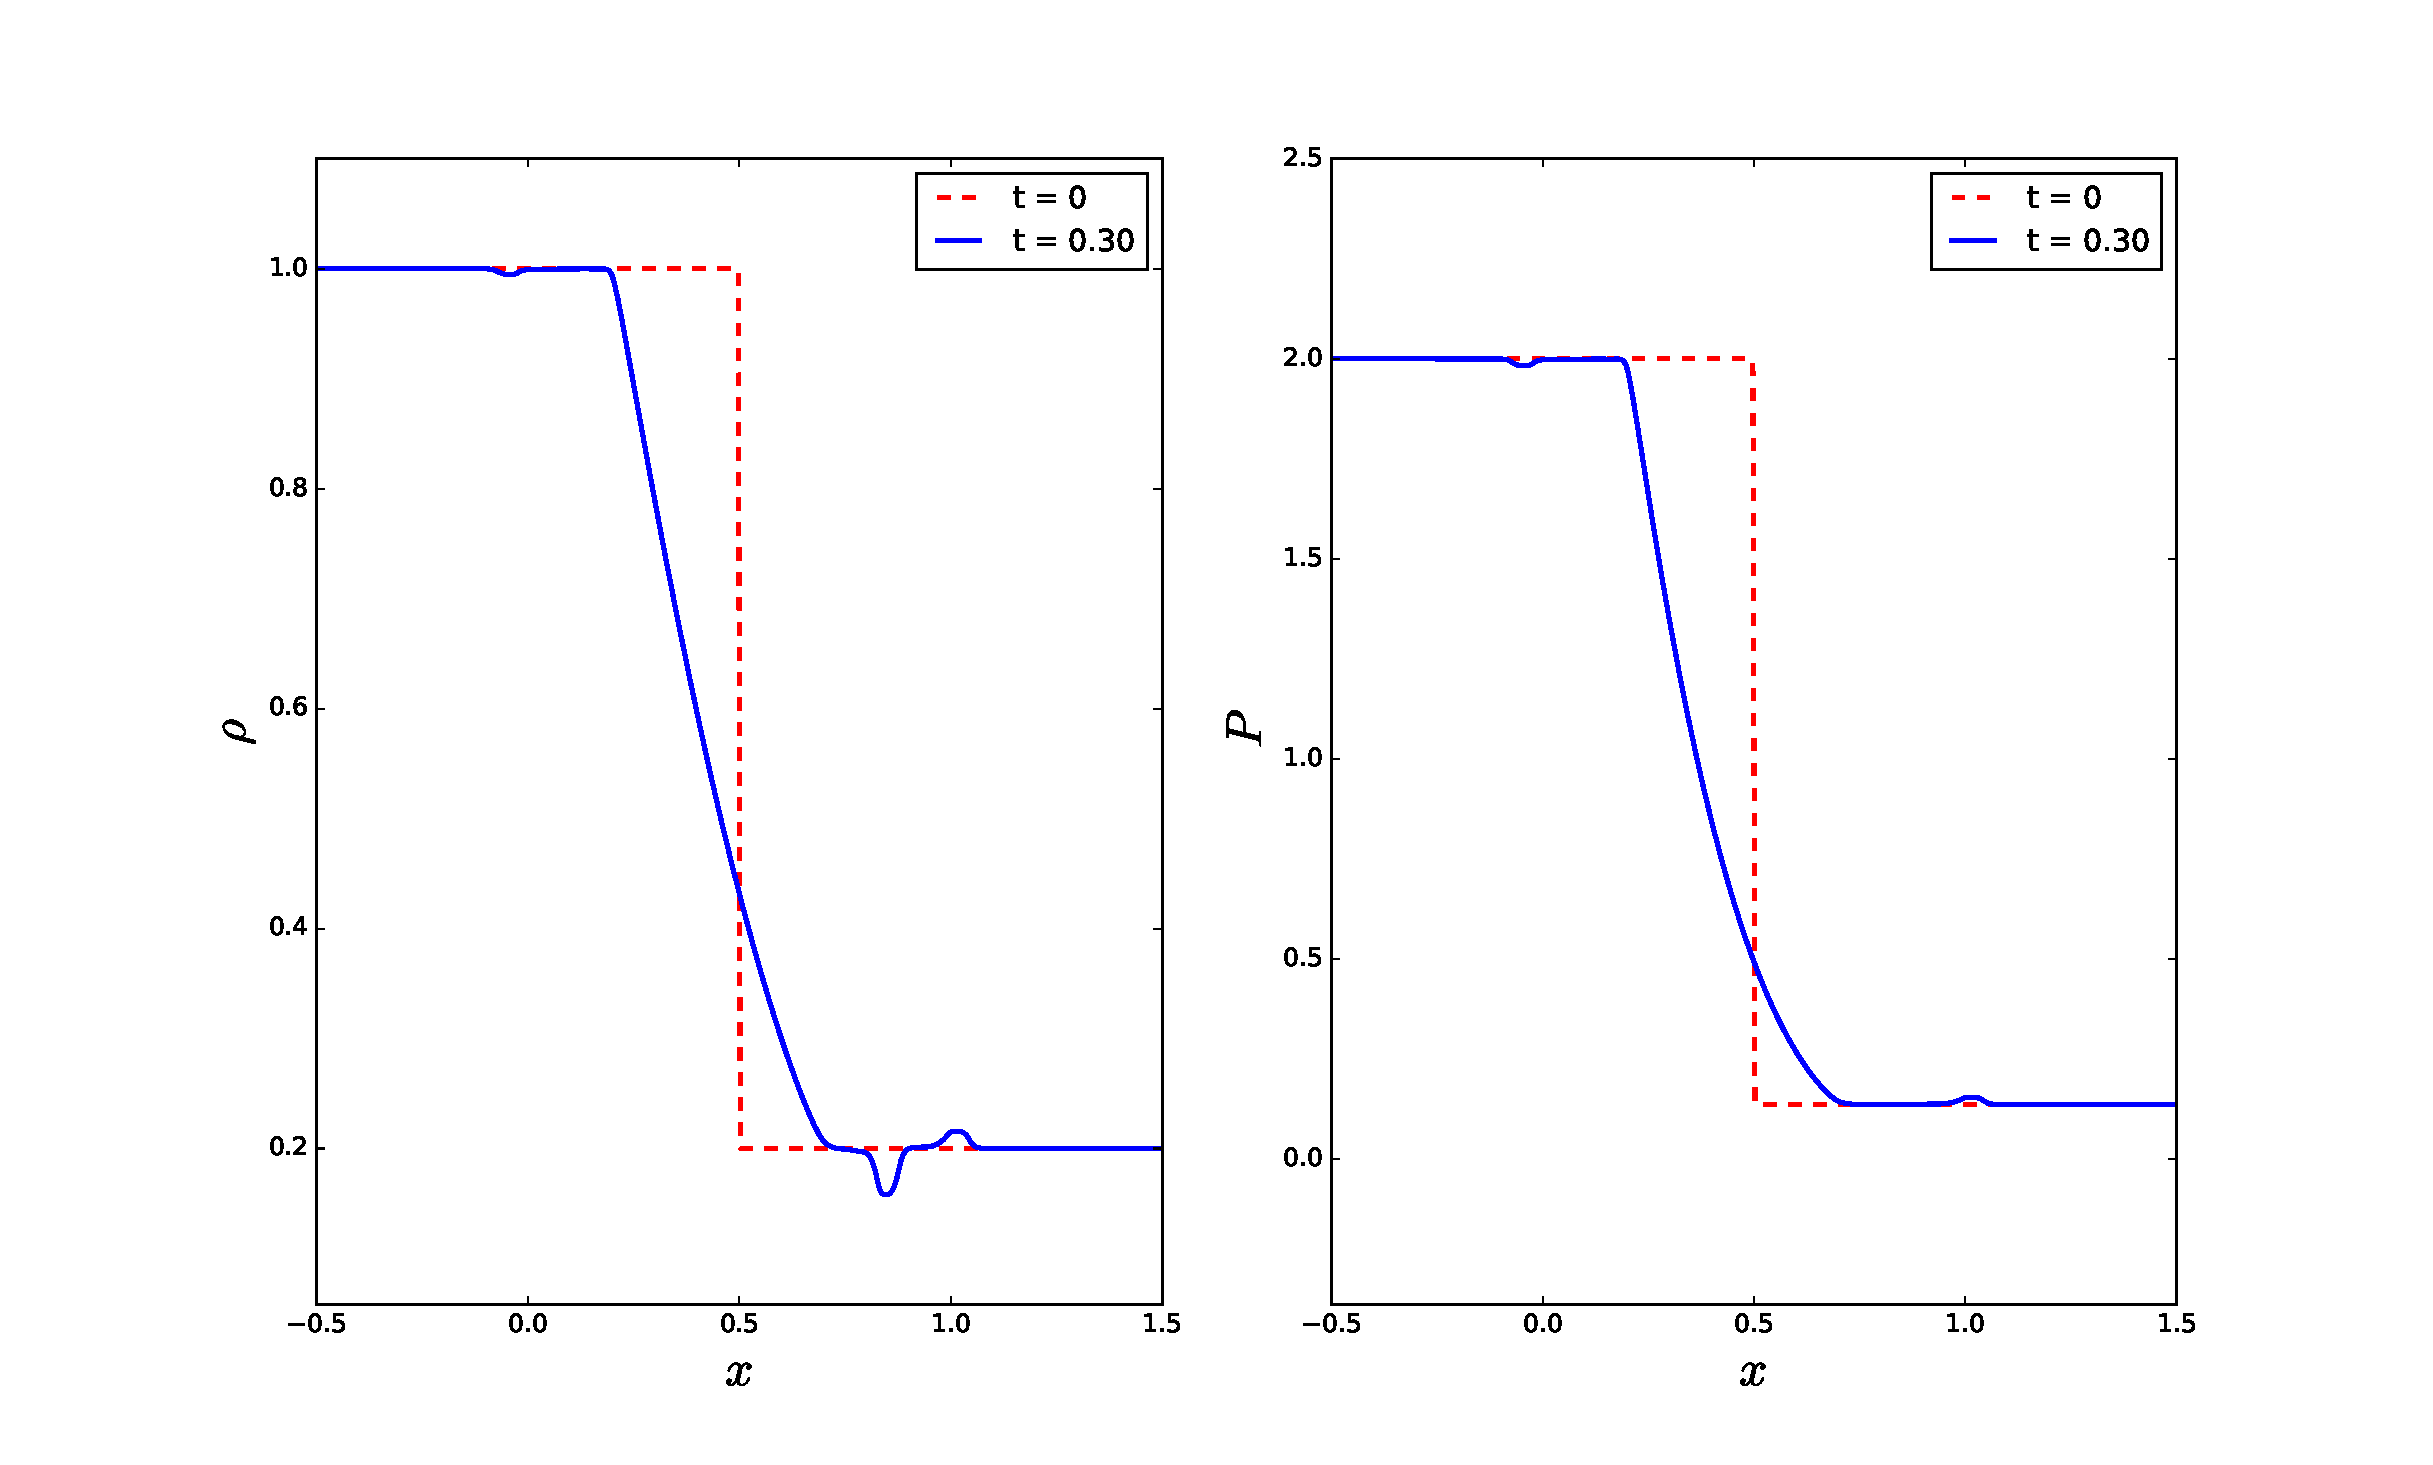
\includegraphics[width=1\textwidth]{SR1.eps}
	\end{minipage}
	\begin{minipage}[c]{0.9\textwidth}
		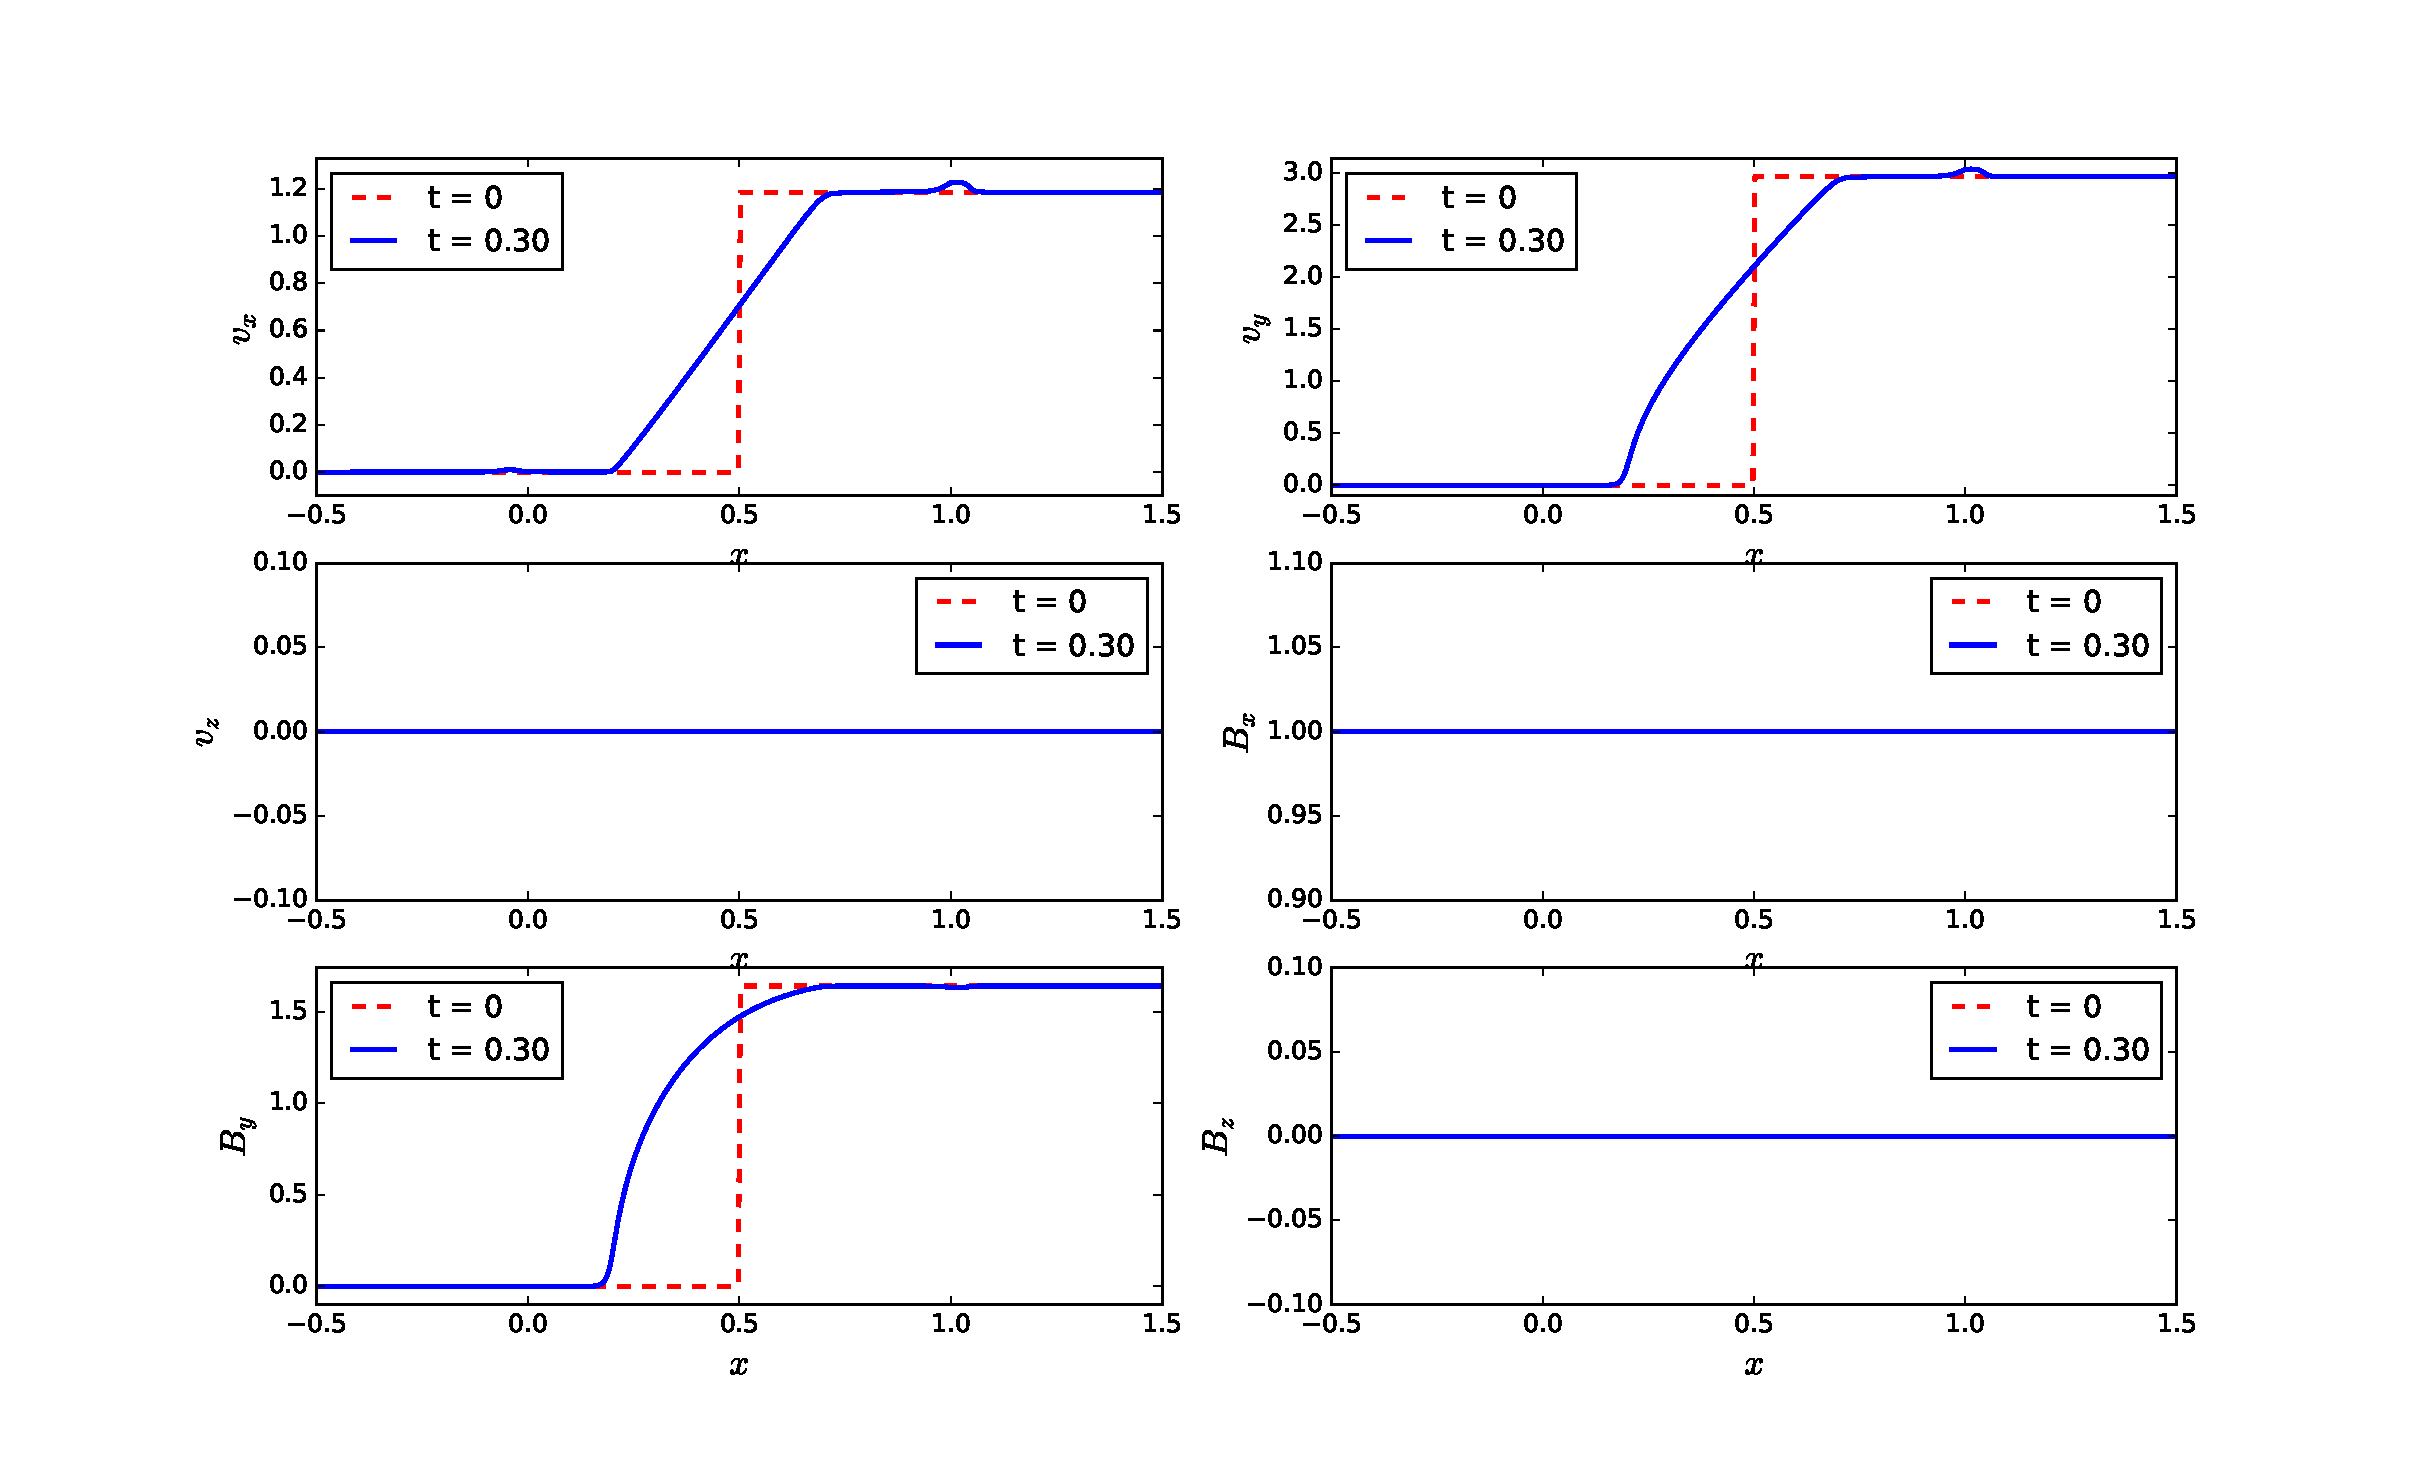
\includegraphics[width=1\textwidth]{SR2.eps}
	\end{minipage}%
\caption{The evolution of SR wave from $t=0$ to $t=0.3$ is plotted. 
The red dashed curves are the initial conditions.}
\label{fig: SR test}
\end{figure}

\section{Conclusions}
My one-dimensional MHD code using PLM + HLL/HLLD scheme is able to 
capture all features of an effective 1D Cartesian MHD system though further promotion is
still possible. It successfully passes all kinds of shock wave and rarefaction wave tests mentioned 
in this work and gives the results similar to those presented in previous papers.

A sinusoidal Alfv\'en wave is constructed and the wave speed of the wave agrees perfectly with 
the theoretical expectation.

For future work, we may check the code carefully to find out a way to promote the accuracy of 
the PLM + HLLD code. Besides, it is interesting to promote this 1D Cartesian code to 
a 1D cylindrical code (in which all physical quantities depend only on the radius $r$), which may be useful for modeling an astrophysical disk and studying its dynamics.

The code would be more useful for real MHD system simulation if we promote it to 
a 3D code like \textit{ATHENA} code \cite{stone2008athena}.

\bibliography{Finalproject_XuYaoHu}


\end{document}